\documentclass[11pt,a4paper]{article}

% ---------------------------------------------------------------------------
% AI651 Assignment 2 -- Questions 1 and 2 (single report)
% Compile with pdfLaTeX (Overleaf default).
% ---------------------------------------------------------------------------
\usepackage[margin=1.8cm]{geometry}
\usepackage[T1]{fontenc}
\usepackage{lmodern}
\usepackage{amsmath,amssymb}
\usepackage{bm}
\usepackage{array}
\usepackage{booktabs}
\usepackage{tabularx}
\usepackage{enumitem}
\usepackage{xcolor}
\usepackage{caption}
\usepackage{float}
\usepackage{graphicx}
\usepackage{makecell}
\usepackage{tikz}
\usetikzlibrary{arrows.meta,positioning,calc}
\usepackage[hidelinks]{hyperref}

\newcolumntype{L}{>{\raggedright\arraybackslash}X}
\setlist{itemsep=1pt,topsep=2pt,parsep=0pt}
\captionsetup{font=small,labelfont=bf,skip=4pt}
\setlength{\parskip}{2pt}

\newcommand{\todo}[1]{\textcolor{red}{\textbf{[#1]}}}
\newcommand{\A}{\mathcal{A}}
\newcommand{\K}{\mathcal{K}}
\newcommand{\Res}{\mathrm{Res}}

\begin{document}

\begin{center}
  {\large Lahore University of Management Sciences}\\[2pt]
  AI651 -- Deep Learning for Space, Time and Graphs \quad (Fall 2026)\\[8pt]
  {\LARGE\bfseries Assignment 2}\\[8pt]
  \begin{tabular}{rl}
    \textbf{Name:} & Muhammad Sikander Raheem \\
    \textbf{Roll number:} & 25280017 \\
    \textbf{GitHub repository:} & \url{https://github.com/sikanderraheem21/DL4TSG_PA2}
  \end{tabular}
\end{center}

\tableofcontents

% ===========================================================================
\section{Question 1 -- River Forecasting Proposal}
% ===========================================================================
\renewcommand{\thefigure}{Q1.\arabic{figure}}
\renewcommand{\thetable}{Q1.\arabic{table}}

\noindent\textbf{Summary.} We propose a \emph{directed river-graph forecaster}.
Every source (stations $S_1$--$S_4$, tributary gauge $T_1$, rain gauges
$R_1,R_2$, and the reservoir) is a node of a graph that follows the river's flow.
A shared causal temporal encoder summarises each node's last 24\,h. Each
station then uses \emph{lag-attention} over all upstream nodes, restricted to
physically plausible travel-time windows. The reservoir node also carries the
schedule announced for the next hour. The output is the change from the last
observed level, as 10/50/90\% quantiles at 10--60\,min. The model is small, so
the 10-minute cycle is easy to meet.


\subsection{Architecture diagram}
% ===========================================================================
Notation: $B$ = batch (issuance times), $W=144$ history steps (24\,h), $F=6$
announced future steps, $H=6$ horizons, $d=64$ hidden width, $N=8$ nodes.

\begin{figure}[H]
\centering
\resizebox{0.97\textwidth}{!}{%
\begin{tikzpicture}[
  font=\small,
  src/.style={draw, rounded corners=2pt, fill=blue!6, align=center,
              text width=2.9cm, minimum height=1.3cm},
  blk/.style={draw, rounded corners=2pt, fill=gray!8, align=center,
              text width=13.0cm, minimum height=1.15cm, inner sep=4pt},
  side/.style={draw, rounded corners=2pt, fill=orange!12, align=center,
               text width=2.9cm, minimum height=1.15cm},
  out/.style={draw, rounded corners=2pt, fill=green!10, align=center,
              text width=2.9cm, minimum height=1.15cm},
  arr/.style={-{Stealth[length=2.2mm]}, thick},
  dim/.style={font=\footnotesize, fill=white, inner sep=1.5pt, align=center},
]
% ---- data sources --------------------------------------------------------
\node[src] (lev)  at (-6.8,0) {Water levels\\$S_1$--$S_4$, $T_1$\\(every 10 min)};
\node[src] (rain) at (-3.4,0) {Rainfall\\$R_1$, $R_2$\\(+ gauge locations)};
\node[src] (rel)  at ( 0.0,0) {Recorded\\reservoir releases};
\node[src] (sch)  at ( 3.4,0) {Announced release\\schedules (announce\\time $a$, effective $e$)};
\node[src] (stat) at ( 6.8,0) {Station locations,\\connectivity,\\river distances};

% ---- alignment ------------------------------------------------------------
\node[blk] (align) at (-1.7,-2.6) {\textbf{As-of-$t_0$ alignment and quality control}\\
  keep only records \emph{received} by $t_0$; snap to the 10-min UTC grid;
  QC (range, spike, flat-line) $\rightarrow$ mask $m$;\\
  forward-fill + age-of-reading $a$; per-channel normalisation;
  latest schedule version with announcement time $\le t_0$};
\node[side] (graph) at (6.8,-2.6) {\textbf{River DAG} $\mathcal{G}$\\
  ancestors $\A(i)$, lag bounds\\ $[\tau^{\min}_{ji},\tau^{\max}_{ji}]$ (A7)};

\foreach \s in {lev,rain,rel,sch}{\draw[arr] (\s.south) -- (\s.south |- align.north);}
\draw[arr] (stat.south) -- (graph.north);

% ---- projection -----------------------------------------------------------
\node[blk] (proj) at (-1.7,-6.0) {\textbf{Type-specific input projection} $W^{\mathrm{in}}_{\mathrm{type}}$
  to width $d=64$, plus node and calendar embeddings;\\
  reshape into node token sequences for
  $\{\Res, R_1, R_2, T_1, S_1, S_2, S_3, S_4\}$ ($N=8$)};

\draw[arr] (align.south -| lev)  -- (proj.north -| lev)
  node[dim,midway] {$\mathbf{X}^{\mathrm{lev}}$\\$B{\times}144{\times}5{\times}3$};
\draw[arr] (align.south -| rain) -- (proj.north -| rain)
  node[dim,midway] {$\mathbf{X}^{\mathrm{rain}}$\\$B{\times}144{\times}2{\times}3$};
\draw[arr] (align.south -| rel)  -- (proj.north -| rel)
  node[dim,midway] {$\mathbf{X}^{\mathrm{rel}}$\\$B{\times}144{\times}1{\times}4$};
\draw[arr] (align.south -| sch)  -- (proj.north -| sch)
  node[dim,midway] {$\mathbf{F}^{\mathrm{rel}}$\\$B{\times}6{\times}1{\times}4$};

% ---- temporal encoder -----------------------------------------------------
\node[blk] (enc) at (-1.7,-8.6) {\textbf{Shared causal dilated TCN}, applied to each node separately:
  7 residual layers, kernel 3, dilations $1,2,\dots,64$\\
  (receptive field 255 $\ge$ 150 steps); keeps one vector \emph{per time step}, so timing is preserved};
\draw[arr] (proj.south) -- (enc.north)
  node[dim,midway] {$\mathbf{U}:\ B{\times}8{\times}T{\times}d$\quad ($T=144$; reservoir: $T=150$ incl.\ 6 announced future steps)};

% ---- lag attention --------------------------------------------------------
\node[blk] (att) at (-1.7,-11.2) {\textbf{Directed lag-attention} (4 heads): for station $i\in\{S_1,\dots,S_4\}$
  and horizon $h$, the query $[\mathbf{z}_i,\mathbf{e}_h]$\\
  attends to tokens $(j,k)$ with $j\in\A(i)\cup\{i\}$ and $k\in\K_{ji}(h)$;
  physically impossible (node, lag) pairs are masked};
\draw[arr] (enc.south) -- (att.north)
  node[dim,midway] {$\mathbf{H}:\ B{\times}8{\times}T{\times}d$};
\draw[arr] (graph.south) |- (att.east) node[dim,pos=0.3] {mask};

% ---- decoder --------------------------------------------------------------
\node[blk] (dec) at (-1.7,-13.8) {\textbf{Decoder}: MLP for each (station, horizon) on
  $[\mathbf{z}_i,\mathbf{m}_{i,h},\mathbf{e}_i,\mathbf{e}_h]$;\\
  forecast = persistence anchor $\ell_i$ + learned change; non-crossing quantiles};
\draw[arr] (att.south) -- (dec.north)
  node[dim,midway] {$\mathbf{M}:\ B{\times}4{\times}6{\times}d$};
\draw[arr,dashed] (enc.west) -- ++(-0.5,0) |- ([yshift=2mm]dec.west)
  node[dim,pos=0.25,left] {$\mathbf{z}_i=\mathbf{H}_{i,0}$};
\draw[arr,dotted] (align.west) -- ++(-1.5,0) |- ([yshift=-2mm]dec.west)
  node[dim,pos=0.2,left] {$\bm{\ell}:\ B{\times}4$\\(last valid level)};

\node[side] (loss) at (6.8,-13.8) {\textit{Training only:}\\ masked pinball loss\\ vs.\ $\mathbf{Y}:\ B{\times}4{\times}6$};
\draw[arr,dashed] (dec.east) -- (loss.west);

% ---- outputs --------------------------------------------------------------
\foreach \x/\n in {-6.8/1,-3.4/2,0/3,3.4/4}{
  \node[out] (o\n) at (\x,-16.4) {$S_{\n}$: level at $t_0{+}60$ min\\ $q_{0.1},\ q_{0.5},\ q_{0.9}$};
  \draw[arr] (dec.south -| o\n) -- (o\n.north);
}
\node[align=left, font=\footnotesize, text width=3.2cm] at (6.9,-16.4)
  {$\hat{\mathbf{Y}}:\ B{\times}4{\times}6{\times}3$\\ (station, horizon $h=1..6$,\\ quantile); served: $h=6$};
\end{tikzpicture}%
}
\caption{Forecasting pipeline. Blue: data sources. Grey: processing blocks.
Orange: the graph prior and the training loss. Green: forecasts. Alignment
puts every source on one 10-minute grid. Projection maps the different
feature types to one width $d$ and reshapes them into one token sequence per
node. Lag-attention combines information across space, using only upstream
nodes at plausible lags.}
\label{fig:arch}
\end{figure}

\begin{figure}[H]
\centering
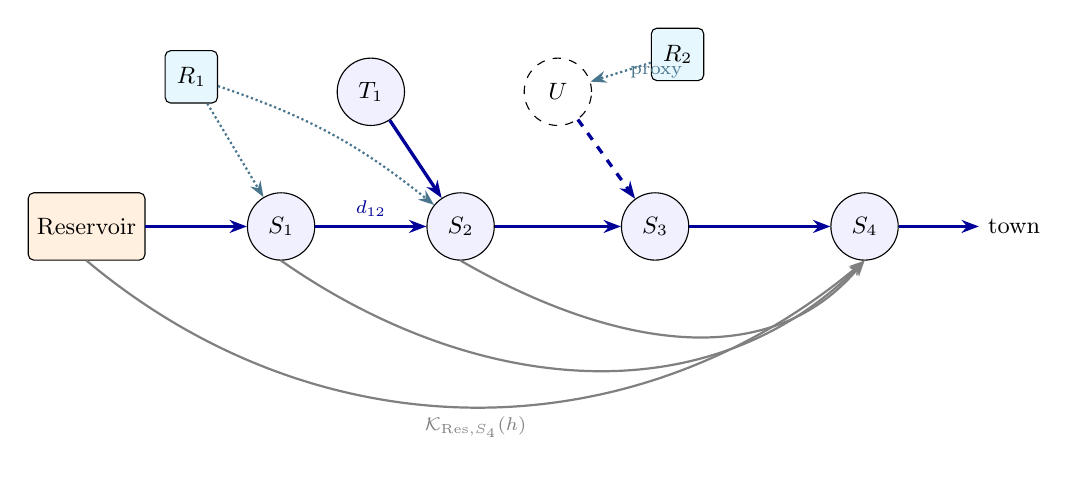
\begin{tikzpicture}[
  font=\small, scale=0.95, transform shape,
  st/.style={draw, circle, minimum size=9mm, fill=blue!6},
  rg/.style={draw, rounded corners=2pt, fill=cyan!10, minimum size=7mm},
  riv/.style={-{Stealth[length=2.2mm]}, very thick, blue!60!black},
  rainarr/.style={-{Stealth[length=2mm]}, densely dotted, thick, cyan!50!black},
  attn/.style={-{Stealth[length=2mm]}, gray, thick},
]
\node[draw, rounded corners=2pt, fill=orange!12, minimum height=9mm] (res) at (0,0) {Reservoir};
\node[st] (s1) at (2.6,0) {$S_1$};
\node[st] (s2) at (5.0,0) {$S_2$};
\node[st] (s3) at (7.6,0) {$S_3$};
\node[st] (s4) at (10.4,0) {$S_4$};
\node (town) at (12.4,0) {town};
\node[st] (t1) at (3.8,1.8) {$T_1$};
\node[draw, dashed, circle, minimum size=9mm] (u) at (6.3,1.8) {$U$};
\node[rg] (r1) at (1.4,2.0) {$R_1$};
\node[rg] (r2) at (7.9,2.3) {$R_2$};

\draw[riv] (res) -- (s1);
\draw[riv] (s1) -- node[above, font=\scriptsize] {$d_{12}$} (s2);
\draw[riv] (s2) -- (s3);
\draw[riv] (s3) -- (s4);
\draw[riv] (s4) -- (town);
\draw[riv] (t1) -- (s2);
\draw[riv, dashed] (u) -- (s3);
\draw[rainarr] (r1) -- (s1);
\draw[rainarr] (r1) to[bend left=10] (s2);
\draw[rainarr] (r2) -- node[right, font=\scriptsize] {proxy} (u);

\draw[attn] (res.south) to[out=-40, in=-140] node[below, font=\scriptsize] {$\K_{\Res,S_4}(h)$} (s4.south);
\draw[attn] (s1.south) to[out=-35, in=-135] (s4.south);
\draw[attn] (s2.south) to[out=-30, in=-130] (s4.south);
\end{tikzpicture}
\caption{River graph $\mathcal{G}$ (schematic). Blue: river flow. Dashed: the
unmonitored tributary $U$, represented in the model by the $R_2$ node (A5,
A11). Dotted: rain drainage. Grey: some of $S_4$'s attention edges. $S_4$
attends directly to all of
$\A(S_4)=\{\Res,S_1,S_2,S_3,T_1,R_1,R_2\}$, each restricted to its own lag
window.}
\label{fig:graph}
\end{figure}

% ===========================================================================
\subsection{Assumptions}
% ===========================================================================
\textbf{Supplied facts.}
\begin{enumerate}[label=\textbf{F\arabic*}, ref=F\arabic*, leftmargin=*]
  \item A forecast is issued every 10\,min, for the level 1\,h ahead at $S_1$--$S_4$.
  \item The reservoir releases upstream of $S_1$, and flow runs $S_1\!\to\!S_4$.
        The monitored tributary ($T_1$) joins between $S_1$ and $S_2$; the
        unmonitored one joins between $S_2$ and $S_3$.
  \item We have 10-minute level histories at $S_1$--$S_4$ and $T_1$; rainfall at
        $R_1$, $R_2$ with timestamps and locations; release records; and
        announced schedules with announcement and effective times.
  \item We have locations, connectivity and along-river distances. Spacing is
        uneven, and travel times vary.
  \item \emph{Not supplied:} travel times, or the unmonitored inflow.
        \emph{Not available at issuance:} future rainfall or future levels.
\end{enumerate}

\noindent\textbf{Assumptions} (statement; \emph{why}; \emph{effect on the design}).
\begin{enumerate}[label=\textbf{A\arabic*}, ref=A\arabic*, leftmargin=*]
  \item \textbf{Record length:} at least 3 years of overlapping data, including
  several floods. \emph{Why:} telemetry is normally archived.
  \emph{Effect:} about $1.5\times10^5$ issuance times, enough for a model of
  about $2\times10^5$ parameters.

  \item \textbf{Time base:} timestamps can be converted to UTC. Levels are
  instantaneous readings, and rain is the depth over the preceding 10\,min.
  Readings lie within $\pm5$\,min of the grid. \emph{Why:} this is standard for
  telemetry. \emph{Effect:} we align by snapping to the grid, with no temporal
  interpolation.

  \item \textbf{Delays:} most readings arrive within 5\,min, but outages can
  delay them by hours. Arrival times are logged. \emph{Why:} this is typical,
  and the brief does not specify delays. \emph{Effect:} features are built as of
  $t_0$, with an age channel and simulated delays (Section~\ref{sec:ops}).

  \item \textbf{Quality:} levels are accurate to $\pm2$\,cm, with spikes,
  flat-lines and up to 10\% gaps. Datums are fixed or documented.
  \emph{Why:} these are common sensor failure modes. \emph{Effect:} quality
  control turns bad readings into missing ones, every input carries a mask,
  and bad targets are excluded from the loss.

  \item \textbf{Rain gauges:} $R_1$ represents the slopes draining to the reach
  between the reservoir and $S_2$; $R_2$ represents the unmonitored
  tributary's catchment. \emph{Why:} these are the nearest gauges in the
  illustration. \emph{Effect:} this fixes the rain edges
  (Figure~\ref{fig:graph}). Attention learns how much each edge matters, so a
  wrong assignment degrades accuracy rather than breaking the model.

  \item \textbf{One-way influence:} levels are controlled from upstream, and
  backwater is negligible. \emph{Why:} it is a steep mountain river.
  \emph{Effect:} stations attend only to their ancestors (U8 covers the case
  where this fails).

  \item \textbf{Travel times:} wave celerity is $c\in[0.5,5]$\,m/s, so
  $\tau_{ji}\in[d_{ji}/c_{\max},\,d_{ji}/c_{\min}]$, and travel time shortens
  as flow rises. \emph{Why:} these are typical kinematic-wave
  speeds~\cite{chow}, widened because the true values are unknown.
  \emph{Effect:} physics fixes the lag-window bounds (Eq.~\ref{eq:window}),
  and the model learns the actual lag.

  \item \textbf{History window:} 24\,h covers the longest travel time, the rain
  response ($\le$12\,h) and one daily cycle. \emph{Why:} this can be checked
  against the supplied distances via
  $W\Delta=\max(24\,\mathrm{h},\tau^{\max}_{\Res,S_4}+6\,\mathrm{h})$.
  \emph{Effect:} $W=144$.

  \item \textbf{Releases:} records give the total outflow within 10\,min.
  Schedules are piecewise-constant, usually followed, but sometimes deviate.
  Past schedule versions are archived with their announcement times.
  \emph{Why:} this is standard gated-reservoir practice, and F3 states that
  announcement times exist. \emph{Effect:} a reservoir node with future steps;
  actual and scheduled channels; and training on the schedule as it was known.

  \item \textbf{$T_1$} lies near the confluence, so its level tracks the
  tributary's inflow. \emph{Effect:} $T_1$ is an ancestor of $S_2$--$S_4$,
  with a short lag window.

  \item \textbf{Unmonitored inflow} is a slow baseflow plus a response to rain
  over its catchment. \emph{Why:} rain is its only observable driver.
  \emph{Effect:} the $R_2$ node stands in for it, and $S_3$'s own history
  captures the baseflow.

  \item \textbf{Slow changes:} channel geometry, operating rules, snowmelt and
  evaporation change slowly compared with one hour and the retraining
  interval. \emph{Effect:} one model, retrained periodically, with calendar
  features and persistence covering the daily and seasonal cycles.

  \item \textbf{Target:} the target is the water level in metres above each
  station's datum. Alert levels $\theta_i$ are known; otherwise we use each
  station's 95th percentile. \emph{Effect:} no rating curve is needed, and the
  loss weights high water (Eq.~\ref{eq:loss}).

  \item \textbf{Infrastructure:} a server reads the telemetry in near real time
  and can publish within 2\,min. \emph{Effect:} the feasibility argument in
  Section~\ref{sec:ops}.
\end{enumerate}

% ===========================================================================
\subsection{Forecasting task and data specification}\label{sec:task}
% ===========================================================================
\textbf{Issuance time:} with $\Delta=10$\,min, a forecast is issued at every
grid time $t_0$ (UTC). $t_0$ is the data cut-off: only records \emph{received}
by $t_0$ are used. The forecast is published by $t_0+2$\,min.

\textbf{History window:} $k\in\{-143,\dots,0\}$, where step $k$ is time
$t_0+k\Delta$ (24\,h).

\textbf{Horizon:} $h\in\{1,\dots,6\}$, valid at $t_0+h\Delta$. The service
output is $h=6$ ($t_0+60$\,min). The other horizons add supervision.

\textbf{Outputs:} quantiles $q\in\mathcal{Q}=\{0.1,0.5,0.9\}$ of
$y_i(t_0+h\Delta)$ for $i\in\{S_1,\dots,S_4\}$.

\textbf{Batch:} one training sample is one issuance time, and $B$ indexes
them. In operation, $B=1$.

\begin{table}[H]
\centering\small
\caption{Model inputs and outputs.}
\label{tab:io}
\begin{tabularx}{\textwidth}{@{}l l L L@{}}
\toprule
\textbf{Tensor} & \textbf{Shape} & \textbf{Axes and content} & \textbf{Time coverage} \\
\midrule
$\mathbf{X}^{\mathrm{lev}}$ & $B\times144\times5\times3$ &
batch, step $k$, gauge ($S_1..S_4,T_1$), feature (level, forward-filled; mask $m$; age $a$) &
$(t_0-24\,\mathrm{h},\,t_0]$; records received by $t_0$ \\
$\mathbf{X}^{\mathrm{rain}}$ & $B\times144\times2\times3$ &
batch, step, gauge ($R_1,R_2$), feature (10-min depth; mask; age) &
step $k$ covers $(t_0+(k-1)\Delta,\,t_0+k\Delta]$ \\
$\mathbf{X}^{\mathrm{rel}}$ & $B\times144\times1\times4$ &
batch, step, reservoir, feature (recorded release; release scheduled for that step; record mask; minutes since announcement) &
$k=-143..0$; mean over each step \\
$\mathbf{F}^{\mathrm{rel}}$ & $B\times6\times1\times4$ &
the same features for future steps; the record slot holds the schedule, with mask 0 &
$(t_0,\,t_0+60\,\mathrm{min}]$; versions with $a\le t_0$ \\
$\mathbf{X}^{\mathrm{cal}}$ & $B\times150\times4$ &
batch, step, $\sin/\cos$ of time of day and day of year &
$k=-143..6$ \\
$\mathcal{G}$ & $23\times3$ &
edge $j\!\to\!i$ (ancestors and self-loops), ($d_{ji},\tau^{\min}_{ji},\tau^{\max}_{ji}$) &
static \\
$\bm{\ell}$ & $B\times4$ & batch, station: last valid level & latest valid reading by $t_0$ \\
\midrule
$\hat{\mathbf{Y}}$ (output) & $B\times4\times6\times3$ &
batch, station, horizon $h$, quantile &
$t_0+h\Delta$; served: $h=6$ \\
$\mathbf{Y},\mathbf{M}^{Y}$ & $B\times4\times6$ & observed future levels and their QC mask (training only) & $t_0+10..60$\,min \\
\bottomrule
\end{tabularx}
\end{table}

\textbf{Alignment across sampling times:} all series are mapped to one
10-minute UTC grid.
\begin{itemize}
  \item \textbf{Levels:} the latest valid reading within $\pm5$\,min of each
        grid time; otherwise the slot is marked missing.
  \item \textbf{Rain:} summed into the slot that ends at each grid time.
  \item \textbf{Releases:} averaged over each slot.
  \item \textbf{Schedules:} indexed by effective time $e$, and filtered by
        announcement time $a\le t_0$.
\end{itemize}

\textbf{Alignment across locations:} we do not interpolate in space. Each
source keeps its own token sequence as a node of $\mathcal{G}$, and the
distances become lag-window bounds and edge features. A type-specific
projection maps the different units and feature counts to width $d$.

\textbf{Available at issuance:} records received by $t_0$, and schedules
announced by $t_0$ (including those effective in $(t_0,t_0+60]$).
\textbf{Not available:} future levels and rain; actual future releases;
schedule changes announced after $t_0$; the unmonitored inflow; and readings
delayed past $t_0$.

% ===========================================================================
\subsection{Model computations and design justification}\label{sec:model}
% ===========================================================================
\textbf{Notation.} Nodes are
$\mathcal{V}=\{\Res,R_1,R_2,T_1,S_1,S_2,S_3,S_4\}$, and
$\mathcal{S}=\{S_1,\dots,S_4\}$ are the stations. $\A(i)$ is the set of nodes
whose water or rain reaches station $i$ (A5, A6):
$\A(S_1)=\{\Res,R_1\}$, $\A(S_2)=\A(S_1)\cup\{S_1,T_1\}$,
$\A(S_3)=\A(S_2)\cup\{S_2,R_2\}$, $\A(S_4)=\A(S_3)\cup\{S_3\}$.
$\mathbf{x}_{j,k}$ is node $j$'s feature vector at step $k$
(Table~\ref{tab:io}). Observed nodes have $k\le0$; the reservoir also has
$k=1..6$, from its schedule. $\mathbf{e}_j$, $\mathbf{e}^{\mathrm{cal}}_k$ and
$\mathbf{e}_h$ are learned node, calendar and horizon embeddings.

\paragraph{(1) Projection and temporal encoder.} Each node's inputs are
projected to width $d$ and passed through a causal dilated TCN~\cite{tcn},
whose weights are shared across nodes. With
$\mathbf{h}^{(0)}_{j,k}=\mathbf{u}_{j,k}$ and dilation $\delta_l=2^{l-1}$:
\begin{equation}
\begin{aligned}
  \mathbf{u}_{j,k} &= W^{\mathrm{in}}_{\mathrm{type}(j)}\mathbf{x}_{j,k} + \mathbf{e}_j + \mathbf{e}^{\mathrm{cal}}_k,\\
  \mathbf{h}^{(l)}_{j,k} &= \mathbf{h}^{(l-1)}_{j,k}
  + W^{(l)}_{o}\,\mathrm{GELU}\Big(\mathrm{LN}\Big(\textstyle\sum_{m=0}^{2}
     W^{(l)}_{m}\mathbf{h}^{(l-1)}_{j,\,k-m\delta_l}\Big)\Big),\quad l=1..7.
\end{aligned}
  \label{eq:tcn}
\end{equation}
Here $\mathbf{H}_{j,k}=\mathbf{h}^{(7)}_{j,k}$, and
$\mathbf{z}_i=\mathbf{H}_{i,0}$ is station $i$'s latest state. Earlier steps
are zero-padded. The receptive field is 255 steps, which covers the window,
and every output depends only on steps $\le k$.

\paragraph{(2) Physically bounded lag windows.} Water that reaches $i$ at
$t_0+h\Delta$ passed $j$ about $\tau_{ji}$ earlier. Using the bounds from A7,
the allowed steps of $j$ for forecast $(i,h)$ are
\begin{equation}
  \K_{ji}(h)=\big\{k:\ h-\lceil\tau^{\max}_{ji}/\Delta\rceil-\kappa \le k \le h-\lfloor\tau^{\min}_{ji}/\Delta\rfloor\big\}\cap\{k\le k^{\max}_j\}.
  \label{eq:window}
\end{equation}
\begin{itemize}
  \item $\kappa=3$ is a margin for attenuation of the wave.
  \item $k^{\max}_j=0$ for observed nodes; $k^{\max}_{\Res}=6$, because the
        schedule is known.
  \item An empty window becomes $\{0\}$: the model extrapolates from the latest
        state.
  \item River edges use $\tau^{\min}=d/c_{\max}$ and $\tau^{\max}=d/c_{\min}$;
        rain edges use $[0,12\,\mathrm{h}]$; self-edges use the last 2\,h.
\end{itemize}
\emph{Example:} with $d_{12}=6$\,km, $\tau_{12}\in[20,200]$\,min, so
$\K_{S_1S_2}(6)=\{-17,\dots,0\}$. The upper bound ($k\le4$) is cut at 0,
because some water that reaches $S_2$ within the hour has not yet passed $S_1$.
This is a physical limit that no model can remove (U2).

\paragraph{(3) Directed lag-attention~\cite{transformer}.} For station $i$ and
horizon $h$, the candidate tokens are
$\mathcal{T}_i(h)=\{(j,k):j\in\A(i)\cup\{i\},\,k\in\K_{ji}(h)\}$. For each head
$r=1..4$:
\begin{equation}
\begin{aligned}
  \alpha^{(r)}_{i,h}(j,k)&=\operatorname*{softmax}_{(j,k)\in\mathcal{T}_i(h)}
   \frac{\big(W^{(r)}_Q[\mathbf{z}_i\|\mathbf{e}_h]\big)^{\!\top} W^{(r)}_K\mathbf{c}_{j,k}}{\sqrt{d/4}},\\
  \mathbf{m}_{i,h}&=W_O\Big\Vert_{r=1}^{4}\sum_{(j,k)\in\mathcal{T}_i(h)}\alpha^{(r)}_{i,h}(j,k)\,W^{(r)}_V\mathbf{c}_{j,k},
\end{aligned}
  \label{eq:attn}
\end{equation}
where $\mathbf{c}_{j,k}=[\mathbf{H}_{j,k}\,\|\,\psi(h-k,d_{ji},j)]$, and $\psi$
is an MLP that encodes the lag, the distance and the source type. Tokens
outside $\mathcal{T}_i(h)$ get zero weight; this is where the physics enters
as a hard constraint.

\paragraph{(4) Forecast mapping.} The decoder computes
$(\delta,a,b)_{i,h}=\mathrm{MLP}([\mathbf{z}_i\|\mathbf{m}_{i,h}\|\mathbf{e}_i\|\mathbf{e}_h])$,
anchored on the last valid level $\ell_i$:
\begin{equation}
  \hat y^{0.5}_{i,h}=\ell_i+\sigma_i\delta_{i,h},\quad
  \hat y^{0.1}_{i,h}=\hat y^{0.5}_{i,h}-\sigma_i\,\mathrm{softplus}(a_{i,h}),\quad
  \hat y^{0.9}_{i,h}=\hat y^{0.5}_{i,h}+\sigma_i\,\mathrm{softplus}(b_{i,h}),
  \label{eq:out}
\end{equation}
Here $\sigma_i$ is the standard deviation of station $i$'s 1-hour level change.
The softplus terms make the quantiles non-crossing. Together,
Eqs.~(\ref{eq:tcn})--(\ref{eq:out}) define the forecast mapping
$\hat{\mathbf{Y}}=f_\theta(\mathbf{X}^{\mathrm{lev}},\mathbf{X}^{\mathrm{rain}},\mathbf{X}^{\mathrm{rel}},\mathbf{F}^{\mathrm{rel}},\mathbf{X}^{\mathrm{cal}};\mathcal{G})$.

\paragraph{(5) Training objective.} A masked pinball loss~\cite{koenker}, with
$\rho_q(e)=\max(qe,(q-1)e)$:
\begin{equation}
  \mathcal{L}(\theta)=\frac{1}{\sum M^{Y}}\sum_{b,i,h}M^{Y}_{b,i,h}\,w_h\,\omega_{b,i,h}
  \sum_{q\in\mathcal{Q}}\rho_q\Big(\frac{y_{b,i,h}-\hat y^{q}_{b,i,h}}{\sigma_i}\Big)+\lambda\|\theta\|^2,
  \label{eq:loss}
\end{equation}
\begin{itemize}
  \item $w_6=2$ and $w_{h<6}=1$, so the served horizon counts most.
  \item $\omega=1+4\cdot\mathbf{1}[y>\theta_i]$ gives extra weight to floods
        (A13).
  \item \textbf{Protocol:} chronological train/validation/test split by year;
        Adam with early stopping on the validation loss at $h=6$; masking and
        delay augmentation; a 5-seed ensemble.
  \item \textbf{Size:} about $1.9\times10^5$ parameters.
  \item \textbf{Deployment test:} the model must beat persistence and
        schedule-aware linear routing at $h=6$, especially on floods.
\end{itemize}

\begin{table}[H]
\centering\small
\caption{How each driver reaches the forecasts.}
\label{tab:drivers}
\begin{tabularx}{\textwidth}{@{}l L l@{}}
\toprule
\textbf{Driver} & \textbf{Path in the model} & \textbf{Affects} \\
\midrule
Upstream levels & tokens of upstream $S_j$ in $\K_{ji}(h)$; the weight peaks at the current travel time & $S_2$--$S_4$ \\
Monitored tributary & $T_1$ tokens, with a short window (A10) & $S_2$--$S_4$ \\
Unmonitored tributary & $R_2$ tokens (its catchment's rain), plus $S_3$'s own history (baseflow) & $S_3,S_4$ \\
Rainfall & past $R_1/R_2$ tokens within the response window; future rain is unknown & $R_1$: all; $R_2$: $S_3,S_4$ \\
Reservoir & recorded releases ($k\le0$) and the announced schedule ($k=1..6$), at distance-based lags & all; fastest at $S_1$ \\
Own state & self-tokens (last 2\,h) and the anchor $\ell_i$ & each \\
\bottomrule
\end{tabularx}
\end{table}

\textbf{Physical assumptions and learned mappings.} \emph{Imposed by physics:}
flow direction (A6); which sources can affect which station (F2, A5);
causality, with only announced schedules as future inputs; travel-time bounds
(A7); and the persistence anchor. \emph{Learned:} the actual lag within each
window and its dependence on flow (through $\mathbf{z}_i$ and
$\mathbf{H}_{j,k}$); attenuation of the wave; the rainfall--runoff response;
tributary contributions, including the unmonitored one; nonlinear
relationships between stations; and the width of the uncertainty.
We use no separate simulator: physics enters as structure, not as equations to
solve. This stays robust when travel times and inflows are unknown.

\textbf{Justification.}
\begin{enumerate}[label=\textbf{J\arabic*}, ref=J\arabic*, leftmargin=*]
  \item \textbf{Spatial input is necessary.} In the companion notebook,
  temporal-only models give one forecast for identical local histories. That
  forecast is the mean (MSE) or median (MAE) of the possible outcomes. An
  upstream rise that has not yet arrived is exactly such a case.

  \item \textbf{Keep timing.} Telling which node saw a rise first needs one
  vector per time step (Think about 2), so the TCN does not pool over time.

  \item \textbf{Reach.} One local S--T pair or ST block reaches 1 node and 2
  steps (Think about 3). The reservoir is 4 hops and tens of steps from $S_4$.
  Direct ancestor edges with attention give full reach in one layer, as
  attention did over a 3-block ST stack in the relay experiment (Think about 4).

  \item \textbf{Mask the attention.} Full attention over $L=1200$ tokens costs
  $2L^2d\approx1.8\times10^8$ operations, which is affordable. But it allows
  physically impossible dependencies, which are a real risk with few floods
  (A1). Masking keeps the reach and encodes what we know.

  \item \textbf{Direct multi-horizon outputs and a persistence anchor.} There is
  no error accumulation from autoregressive feedback, and the announced future
  enters naturally, as in TFT~\cite{tft}. The model's capacity goes to events
  rather than to steady periods.

  \item \textbf{Quantiles.} Under missing information, MSE returns a mean that
  may be implausible (Think about 1). Quantiles give the median and a
  calibrated range, which is what flood preparedness needs.

  \item \textbf{Alternatives.} A per-station LSTM cannot see upstream.
  Neighbour-only GNNs (DCRNN~\cite{dcrnn}, Graph WaveNet~\cite{gwn}) need
  several hops. Pure Muskingum routing~\cite{chow} needs travel times and
  inflows we do not have. Our design follows data-driven rainfall--runoff
  models~\cite{kratzert}, with a river graph added.
\end{enumerate}

% ===========================================================================
\subsection{Operation and exceptional conditions}\label{sec:ops}
% ===========================================================================
\textbf{(i) Missing observations.}
\begin{itemize}
  \item Quality control (A4) marks gaps, out-of-range values, spikes and
        flat-lines as missing.
  \item A missing input is forward-filled, with mask $m=0$ and a growing age
        $a$, so the model knows a reading is stale and by how much.
  \item Training randomly masks 5--20\% of readings, and sometimes whole sensors
        for 1--12\,h. The model therefore learns other paths: for example, if
        $S_2$ is down, $S_3$ leans on $S_1$ and $T_1$ at longer lags.
  \item Missing targets are excluded from the loss.
  \item If a station's own sensor is missing, its anchor is the last valid
        value, its range widens, and the forecast is flagged \emph{degraded}.
  \item After more than 6\,h without data, or if all ancestors are missing, the
        station falls back to persistence plus schedule-aware routing,
        flagged \emph{fallback}.
\end{itemize}

\textbf{(ii) Delayed observations.}
\begin{itemize}
  \item Each record stores its observation time and its arrival time.
  \item Features use an as-of join (arrival $\le t_0$), so a late reading looks
        like a missing reading with growing age. Training simulates delays
        drawn from the logged distribution (A3), so it sees the same
        situation.
  \item The forecast never waits for data.
  \item Late data enters the next issuance, 10\,min later. If it moves the
        60-minute median by more than 5\,cm, an updated forecast is issued
        immediately.
  \item Each forecast's inputs are logged for audit.
\end{itemize}

\textbf{(iii) Announced future releases.}
\begin{itemize}
  \item The reservoir's steps $k=1..6$ come from the latest schedule with
        $a\le t_0$.
  \item Releases effective after $t_0+60$\,min cannot affect the hour, so they
        are excluded.
  \item The lag windows send a release effective at $e$ to station $i$ near
        $e+\tau_{\Res,i}$. A change at $t_0+20$\,min therefore lifts the $S_1$
        forecast only for $t_0+30..60$.
  \item ``Minutes since announcement'' lets the model learn that last-minute
        schedules are less reliable.
  \item Training uses each schedule \emph{as it was known} at $t_0$ (A9), never
        the outcome, so there is no leakage.
\end{itemize}

\textbf{(iv) Scheduled versus actual releases.}
\begin{itemize}
  \item Past reservoir tokens hold both the \emph{recorded} release and the
        release \emph{scheduled} for that step; future tokens hold only the
        schedule.
  \item The model therefore learns typical deviations, such as a late start,
        and the quantiles absorb the rest.
  \item \textbf{Live detection:} $S_1$ sits just below the dam, so a deviation
        appears there first. If the record, or $S_1$'s response, departs from
        the schedule beyond a threshold, the next issuance uses the record, the
        forecast is flagged \emph{schedule deviation}, and the operator is
        asked to confirm.
  \item A missing record is replaced by the schedule, with $m=0$.
  \item An emergency release enters the next issuance as a new schedule version.
\end{itemize}

\textbf{Feasibility.} One issuance ($B=1$, 1200 tokens, $d=64$) costs about
$7\times1200\times4d^2\approx1.4\times10^8$ multiply-adds in the TCN, plus
about $10^7$ for 24 attention queries. That is under 0.3\,GFLOP, or 10--50\,ms
on one CPU core, and the 5-member ensemble stays under 1\,s. Building the
features reads about 1200 values. The full cycle (fetch, quality control,
inference, publish, log) fits easily within 2 minutes. Retraining
($\sim\!1.5\times10^5$ samples) takes minutes on one GPU, run monthly or on
drift. A watchdog restarts failed runs, and the persistence fallback is
published if the model is unavailable.

% ===========================================================================
\subsection{Uncertainty, limitations, and additional information}\label{sec:unc}
% ===========================================================================
Each item gives its impact, our response, and what remains unresolved.
\begin{enumerate}[label=\textbf{U\arabic*}, ref=U\arabic*, leftmargin=*]
  \item \textbf{Unmonitored tributary.} \emph{Impact:} storms over its
  catchment raise $S_3$ and $S_4$ with no upstream warning, so the median
  lags. \emph{Response:} the $R_2$ proxy, $S_3$'s own trend, and wider
  $S_3$/$S_4$ ranges when $R_2$ is wet. \emph{Unresolved:} storms that $R_2$
  misses (D3).

  \item \textbf{Changing travel times.} \emph{Impact:} a fixed lag mistimes
  peaks. \emph{Response:} attention picks the lag from the current state,
  within wide bounds. We check the learned lags against physics on recorded
  events. \emph{Unresolved:} overbank floods may fall outside the bounds
  (D4). On short reaches, water arriving within the hour is partly
  unobserved (Eq.~\ref{eq:window}).

  \item \textbf{Future rain.} \emph{Impact:} rain after $t_0$ on fast slopes
  causes under-prediction. \emph{Response:} ranges that reflect recent rain.
  \emph{Unresolved} without D5.

  \item \textbf{Rare extremes.} \emph{Impact:} networks extrapolate poorly.
  \emph{Response:} the anchor, flood weighting, an ``outside training range''
  flag, and the routing fallback. \emph{Unresolved:} unprecedented floods,
  where forecasts are indicative only.

  \item \textbf{Sparse rain gauges.} \emph{Impact:} two gauges miss rain that
  varies over mountains. \emph{Response:} learned weights and wider ranges
  (D5, D6).

  \item \textbf{Sensor drift and datum shifts.} \emph{Response:} quality
  control, checks against neighbouring stations, and maintenance logs (D1).
  \emph{Unresolved:} slow drift can look like real change.

  \item \textbf{Non-stationarity} (sediment, vegetation, new rules).
  \emph{Response:} monitor rolling error and coverage; retrain monthly or on
  drift (A12).

  \item \textbf{Backwater} at high tributary flows violates A6.
  \emph{Response:} add a downstream edge if validation errors show it.

  \item \textbf{Calibration under shift.} \emph{Response:} conformalised
  quantile recalibration~\cite{cqr} on a rolling window keeps 80\% coverage;
  the ensemble spread adds epistemic uncertainty.

  \item \textbf{Release deviations.} \emph{Response:} Section~\ref{sec:ops}(iv),
  plus telemetry (D2).
\end{enumerate}

\noindent\textbf{Additional information requests.} The system works with the
supplied data alone; each request improves it.

\begin{table}[H]
\centering\small
\caption{Additional information requested.}
\label{tab:requests}
\begin{tabularx}{\textwidth}{@{}l L L l@{}}
\toprule
\textbf{ID} & \textbf{Request} & \textbf{How it helps} & \textbf{Usable without?} \\
\midrule
D1 & Record length, latency logs, QC and maintenance metadata & Confirms A1--A4; realistic delay simulation & Yes (assumed) \\
D2 & Archived schedule versions; gate and spillway telemetry & Training without leakage; early deviation detection & Yes, wider ranges \\
D3 & A gauge, even a temporary one, on the unmonitored tributary & Observes the main unknown; added as a new node, no redesign & Yes, wider $S_3/S_4$ \\
D4 & Cross-sections, travel-time studies, or a hydraulic model & Tighter $[\tau^{\min},\tau^{\max}]$; validates lags; a better fallback & Yes, wide bounds \\
D5 & Radar or rainfall nowcasts for the next hour & Future rain, as a known-future input (U3) & Yes, lower skill \\
D6 & More rain gauges; snow and temperature data & Spatial rain coverage; snowmelt & Yes \\
D7 & Rating curves and discharge data & Mass-balance checks; discharge extension & Yes \\
D8 & Official alert levels and how forecasts are used & Sets $\theta_i$ and which quantile to act on & Yes (95th pct.) \\
\bottomrule
\end{tabularx}
\end{table}


% ===========================================================================
\section{Question 2 -- Motion or Memory?}
% ===========================================================================
\setcounter{figure}{0}\setcounter{table}{0}
\renewcommand{\thefigure}{\arabic{figure}}
\renewcommand{\thetable}{\arabic{table}}

\paragraph{Setup and reproducibility.}
\begin{itemize}
  \item \textbf{Code:} all code is in the repository (\texttt{q2/}). Each table
        and figure is produced by one command, listed in \texttt{README.md}.
  \item \textbf{Data:} Moving MNIST~\cite{srivastava} is loaded with \texttt{split=None} and split
        by video index into train 0--7,999, validation 8,000--8,999 and test
        9,000--9,999.
  \item \textbf{Training:} every learned model is trained with seeds 0 and 1 on
        an NVIDIA \textbf{Tesla T4} (Google Colab, PyTorch 2.11).
  \item \textbf{Evaluation and inference timing:} on an Apple M1 Pro
        \textbf{CPU} (6 threads, PyTorch 2.15), the same machine for every
        model.
  \item \textbf{Reporting:} every learned-model entry is \emph{mean (seed 0,
        seed 1)}. All errors are on the 1,000 test videos unless stated
        otherwise.
  \item \textbf{Pre-registration:} the Q2.5 prediction was committed at
        \texttt{ba0b7e8} (29 Oct, 01:39), before the Testing-the-Baseline
        results (\texttt{9cc1ac4}, 01:48). The Q2.11 prediction was committed at
        \texttt{cbe906a} (01:49), before models B, C and D were trained
        (\texttt{68c081f}, 30 Oct).
\end{itemize}

% ---------------------------------------------------------------------------
\subsection{Setup}

\begin{table}[H]
\centering\small
\caption{Checks of the transformation and window functions, using the functions the experiments call (\texttt{q2/checks.py}).}
\label{tab:q2-checks}
\begin{tabular}{@{}lll@{}}
\toprule
\textbf{Check} & \textbf{Expected} & \textbf{Ours} \\
\midrule
(a) $\max|M(M(x))-x|$ & 0 & 0 (\texttt{torch.equal}: True) \\
(b) $\max|R^4(x)-x|$ & 0 & 0 (\texttt{torch.equal}: True) \\
(c) $\max|MRM(x)-R^{-1}(x)|$ & 0 & 0 (\texttt{torch.equal}: True) \\
(d) bright pixel of $M(p)$ (frame, row, column) & (7, 10, 43) & (7, 10, 43) \\
(e) bright pixel of $R(p)$ (frame, row, column) & (7, 43, 10) & (7, 43, 10) \\
(f) $1\times$ input / target frames & 1--5 / 6--10 & 1--5 / 6--10 \\
(g) $2\times$ input / target frames & 1,3,5,7,9 / 11,13,15,17,19 & 1,3,5,7,9 / 11,13,15,17,19 \\
(h) $3\times$ input / target frames & 1,4,7,10,13 / 16,19 & 1,4,7,10,13 / 16,19 \\
\bottomrule
\end{tabular}
\end{table}

\begin{figure}[H]
\centering
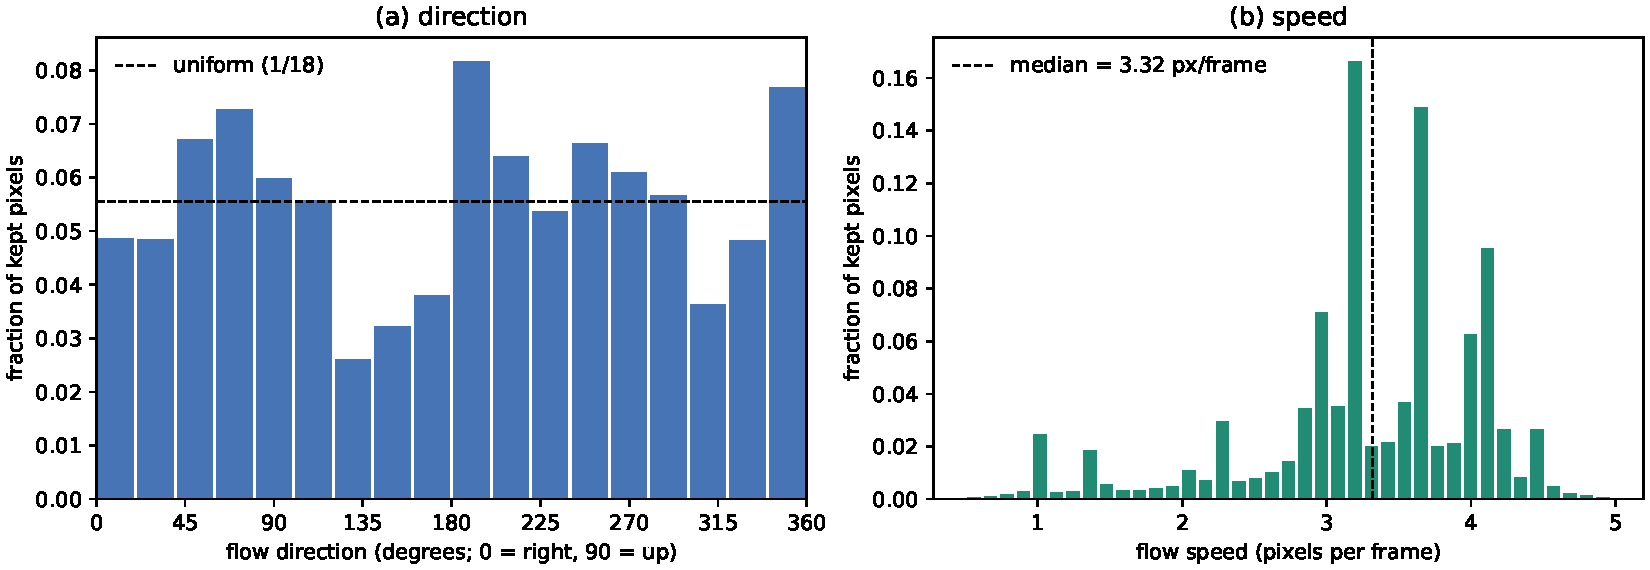
\includegraphics[width=\textwidth]{figures/figure1_optical_flow.pdf}
\caption{Motion statistics of the first 50 training videos (950 frame pairs),
from Farneback optical flow with the handout's settings. We keep pixels
brighter than 0.2 in both frames with flow magnitude above 0.5\,px:
\textbf{103,050 pixels}. (a) Flow direction, as a fraction of kept pixels,
with the uniform level $1/18$ dashed. (b) Flow speed. The \textbf{median is
3.32\,px/frame}; 80\% of speeds lie between 2.14 and 4.12, and the 99th
percentile is 4.67.}
\label{fig:q2-flow}
\end{figure}

\paragraph{Q2.1.} \emph{Familiarity.}
\begin{itemize}
  \item \textbf{Mirror} maps a direction $\theta$ to $180^\circ-\theta$, which
        reflects histogram (a) about $90^\circ$. \textbf{Rotation} maps $\theta$
        to $\theta+90^\circ$, which shifts it by 4.5 bins. Neither changes
        speed.
  \item Every 20$^\circ$ bin already holds 2.6\%--8.2\% of the pixels. So every
        mirrored or rotated direction is a direction the model has seen.
  \item The bins are not uniform, but that is consistent with sampling noise
        from about 100 digit trajectories in 50 videos, rather than a real
        preference for any direction. The generator draws directions at random
        and bounces off all four walls.
  \item So mirrored and rotated \emph{trajectories} should already be familiar.
        What is unfamiliar is the mirrored or rotated \emph{digit shapes}.
\end{itemize}
\emph{Speed.}
\begin{itemize}
  \item A typical digit moves about \textbf{3.3\,px/frame}, with an
        interquartile range of 3.0--3.9.
  \item $2\times$ is about \textbf{6.6\,px} and $3\times$ about
        \textbf{10\,px} between the frames the model sees. Both are far above
        the 99th percentile of the training data (4.7\,px), so fast motion is
        new to the model.
\end{itemize}
\emph{Overlap bias.}
\begin{itemize}
  \item Where digits overlap, Farneback returns a blend of the two velocities.
        Speeds come out smaller, and directions are pulled towards the mean of
        the two digits.
  \item The intensity mask keeps these pixels, so the histograms are slightly
        biased towards lower speeds.
  \item Overlap occupies only a minority of frames and pixels, and a blend
        stays inside the range of true velocities. So it cannot create a
        missing direction, or push a typical speed to $2\times$. The conclusion
        does not change.
\end{itemize}

\paragraph{Q2.2.}
\begin{itemize}
  \item \textbf{Mirror and rotation} change the \textbf{digit appearance} but
        not the \textbf{motion statistics}: speeds are preserved, and the
        direction distribution is (almost) invariant, as shown in Q2.1.
  \item \textbf{Speed-up} changes the \textbf{motion statistics} (speeds triple
        at $3\times$) but not the \textbf{appearance}: the frames are the
        original frames.
\end{itemize}
Each transformation therefore changes one factor while holding the other fixed.
If a model fails under mirror or rotation, the cause is appearance. If it fails
under speed-up, the cause is motion. This is a controlled experiment on a
single trained model, with no retraining.

% ---------------------------------------------------------------------------
\subsection{Baseline: ConvLSTM}

\paragraph{Model A} is the ConvLSTM of~\cite{shi} without peepholes, following
the handout's equations exactly (\texttt{q2/models.py}):
\begin{itemize}
  \item \texttt{pixel\_unshuffle(4)};
  \item two peephole-free ConvLSTM layers (64 channels, $3\times3$, one
        convolution producing all four gates);
  \item a $1\times1$ convolution from 64 to 16 channels, then
        \texttt{pixel\_shuffle(4)} and a sigmoid;
  \item a 9-step rollout with no teacher forcing;
  \item \textbf{480,784} trainable parameters, as specified.
\end{itemize}
The loss is masked to the \emph{available} target frames of each video.

\begin{table}[H]
\centering\small
\caption{Test error at $1\times$, $t=1$ (inputs frames 1--5, targets 6--10).}
\label{tab:q2-baseline}
\resizebox{\textwidth}{!}{%
\begin{tabular}{@{}lccccccr@{}}
\toprule
& MSE$_1$ & MSE$_2$ & MSE$_3$ & MSE$_4$ & MSE$_5$ & $E^{(5)}$ & Params \\
\midrule
Model A & \makecell{0.0173\\(0.018, 0.0166)} & \makecell{0.0206\\(0.0214, 0.0199)} & \makecell{0.0229\\(0.0236, 0.0223)} & \makecell{0.0247\\(0.0252, 0.0242)} & \makecell{0.0264\\(0.0268, 0.0261)} & \makecell{\textbf{0.0224}\\(0.023, 0.0218)} & 480,784 \\
Blank & 0.0426 & 0.0426 & 0.0426 & 0.0425 & 0.0425 & 0.0426 & 0 \\
Copy-last & 0.0492 & 0.0604 & 0.0669 & 0.0708 & 0.0732 & 0.0641 & 0 \\
\bottomrule
\end{tabular}%
}
\end{table}

\begin{figure}[H]
\centering
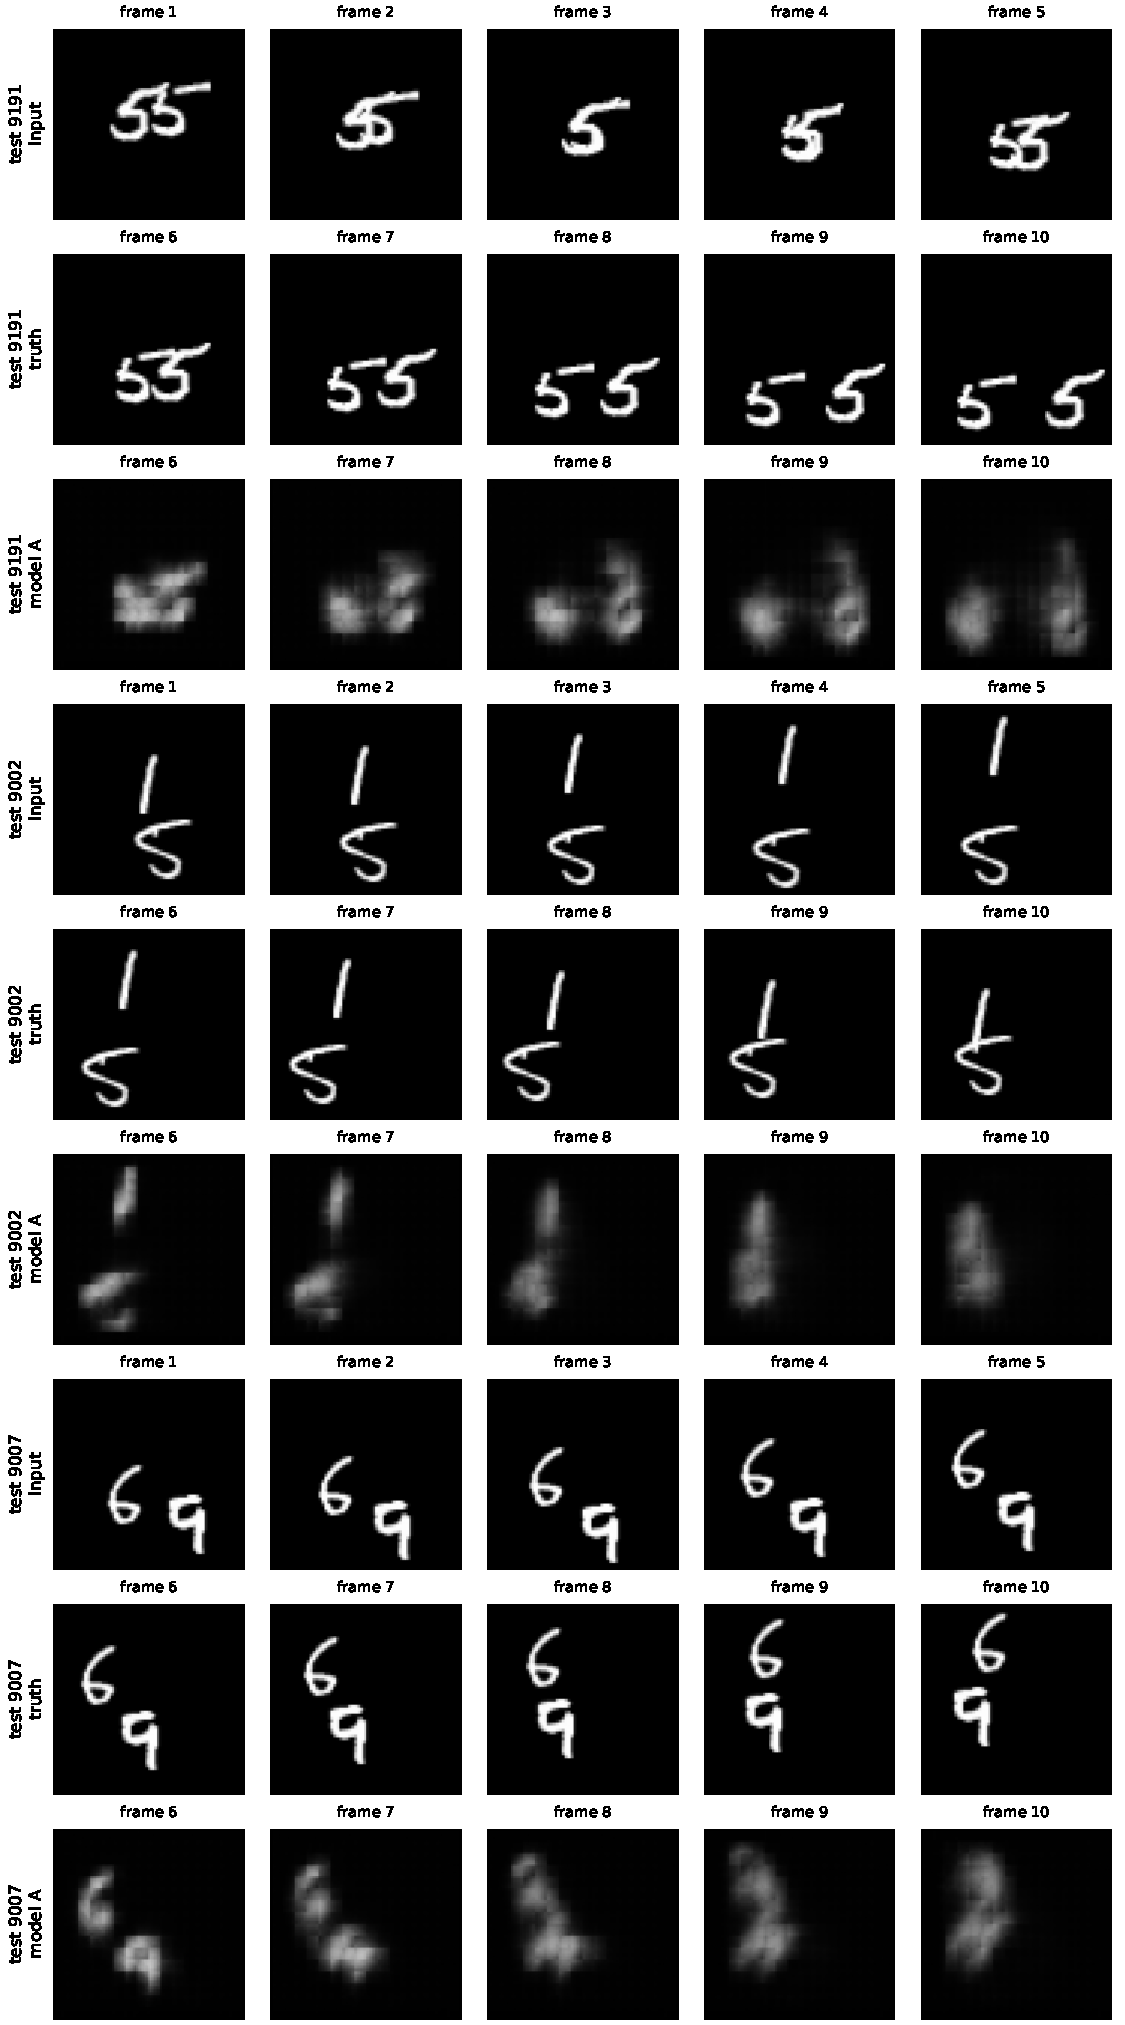
\includegraphics[height=0.62\textheight]{figures/figure2_baseline_examples.pdf}
\caption{Inputs, ground truth and seed-0 model A predictions for three test
videos. Video 9191 has overlapping digits (two 5s). Video 9002's digits meet
at frames 9--10. Video 9007's digits stay apart.}
\label{fig:q2-baseline}
\end{figure}

\paragraph{Q2.3: reach of model A.}
\begin{itemize}
  \item \textbf{Grid size.} After folding, one grid cell is 4 original pixels.
  \item \textbf{What moves information.} Only the two $3\times3$ convolutions
        (stride 1, padding 1, dilation 1) do. Each moves information by 1 cell
        per application. The $1\times1$ readout and the (un)shuffles move
        nothing, and the cell state $c$ is updated pointwise.
  \item \textbf{The paths within step $\tau$:}
  \begin{itemize}
    \item $u_\tau\to$ layer-1 conv $\to h^{(1)}_\tau\to$ layer-2 conv
          $\to h^{(2)}_\tau\to\hat x_{\tau+1}$: 2 convolutions.
    \item $h^{(1)}_{\tau-1}$ enters the same layer-1 convolution (it is
          concatenated with $u_\tau$), then passes through layer 2: 2
          convolutions.
    \item $h^{(2)}_{\tau-1}$ passes only through the layer-2 convolution:
          1 convolution.
    \item $c^{(\ell)}_{\tau-1}$ reaches $h^{(\ell)}_\tau$ pointwise, so it adds
          at most the convolutions downstream of it.
  \end{itemize}
  \item \textbf{Result.} The longest path has 2 convolutions, so
        $\text{reach}=4\,\text{px}\times(1+1)=\textbf{8 px per time step}$.
\end{itemize}
In general, $\text{reach}=\text{patch}\times\sum_\ell d_\ell\lfloor k_\ell/2\rfloor$,
implemented in \texttt{reach\_pixels} in \texttt{q2/models.py}.

\paragraph{Q2.4.} \emph{Against the references.} Model A's $E^{(5)}=0.0224$ is
about half of Blank's (0.0426) and a third of Copy-last's (0.0641). It is better
at every horizon, consistently across both seeds.

\emph{Growth with horizon.} The error rises steadily from 0.0173 at $h=1$ to
0.0264 at $h=5$ (+53\%), but stays below Blank throughout. Figure~2 shows why:
\begin{itemize}
  \item the predictions move in roughly the right direction;
  \item they lose sharpness every step, because the rollout feeds back its own
        blurred outputs;
  \item by frame 10 the digits are smudges. Under MSE, a blurred guess is
        cheaper than a sharp guess in the wrong place.
\end{itemize}
\emph{Overlap.} When the digits overlap (video 9191, and video 9002 at frames
9--10), the model produces \emph{one merged blob} rather than two digits
passing through each other. After the digits separate, it recovers only two
faint blobs without their shapes.

\paragraph{Q2.5 (verbatim, committed at \texttt{ba0b7e8} before any test was run).}
\begin{quote}\small
\textbf{Mirror.} Model A will mostly pass the mirror test. Mirroring maps a motion direction $\theta$ to $180^\circ-\theta$, and Figure 1(a) shows that every direction already occurs in training, so the mirrored motion is familiar. What changes is the digits' appearance: a mirrored 2 or 7 is not a shape the model has seen. I expect E\_M to be somewhat higher than E(5) (roughly 10--30\%), with a small but non-zero consistency gap C\_M. The extra error will show up as blurrier or distorted digits, rather than digits moving the wrong way.

\textbf{Rotation.} Rotation will be harder than mirroring, but it will also not fail completely. A $90^\circ$ rotation shifts every direction by $90^\circ$, which is again a familiar motion, so the motion rule should still carry over. But rotated digits look even less like training digits than mirrored ones, so I expect E\_R $>$ E\_M and C\_R $>$ C\_M. If rotation is worse, I would attribute the difference to appearance, not motion.

\textbf{Speed.} At $1\times$ (about 3.3 px per frame) digits move well within the model's reach of about 8 px per step. At $2\times$ (about 6.6 px) the motion is still inside the reach but faster than almost anything in training (the 99th percentile is 4.7 px), so I expect clear degradation, mainly extra blur and lag, but the digits should still roughly follow their paths. At $3\times$ (about 10 px) digits jump further than information can travel in one step, so model A will break down: I expect digits to stall near their last position, smear out, or fade away, with E(2) at $3\times$ close to or worse than Copy-last.
\end{quote}

% ---------------------------------------------------------------------------
\subsection{Testing the Baseline}

\begin{table}[H]
\centering\small
\caption{Consistency gaps and transformed errors at $1\times$, $t=1$, averaged over pixels, the five horizons and the test videos.}
\label{tab:q2-sym}
\resizebox{\textwidth}{!}{%
\begin{tabular}{@{}lccccc@{}}
\toprule
& $E^{(5)}$ & $C_M$ & $E_M$ & $C_R$ & $E_R$ \\
\midrule
Model A & 0.0224 (0.023, 0.0218) & 1.83e-03 (1.72e-03, 1.94e-03) & 0.023 (0.0235, 0.0225) & 2.98e-03 (2.74e-03, 3.22e-03) & 0.024 (0.0244, 0.0235) \\
Blank & 0.0426 & 0 & 0.0426 & 0 & 0.0426 \\
Copy-last & 0.0641 & 0 & 0.0641 & 0 & 0.0641 \\
\bottomrule
\end{tabular}%
}
\end{table}

\begin{figure}[p]
\centering
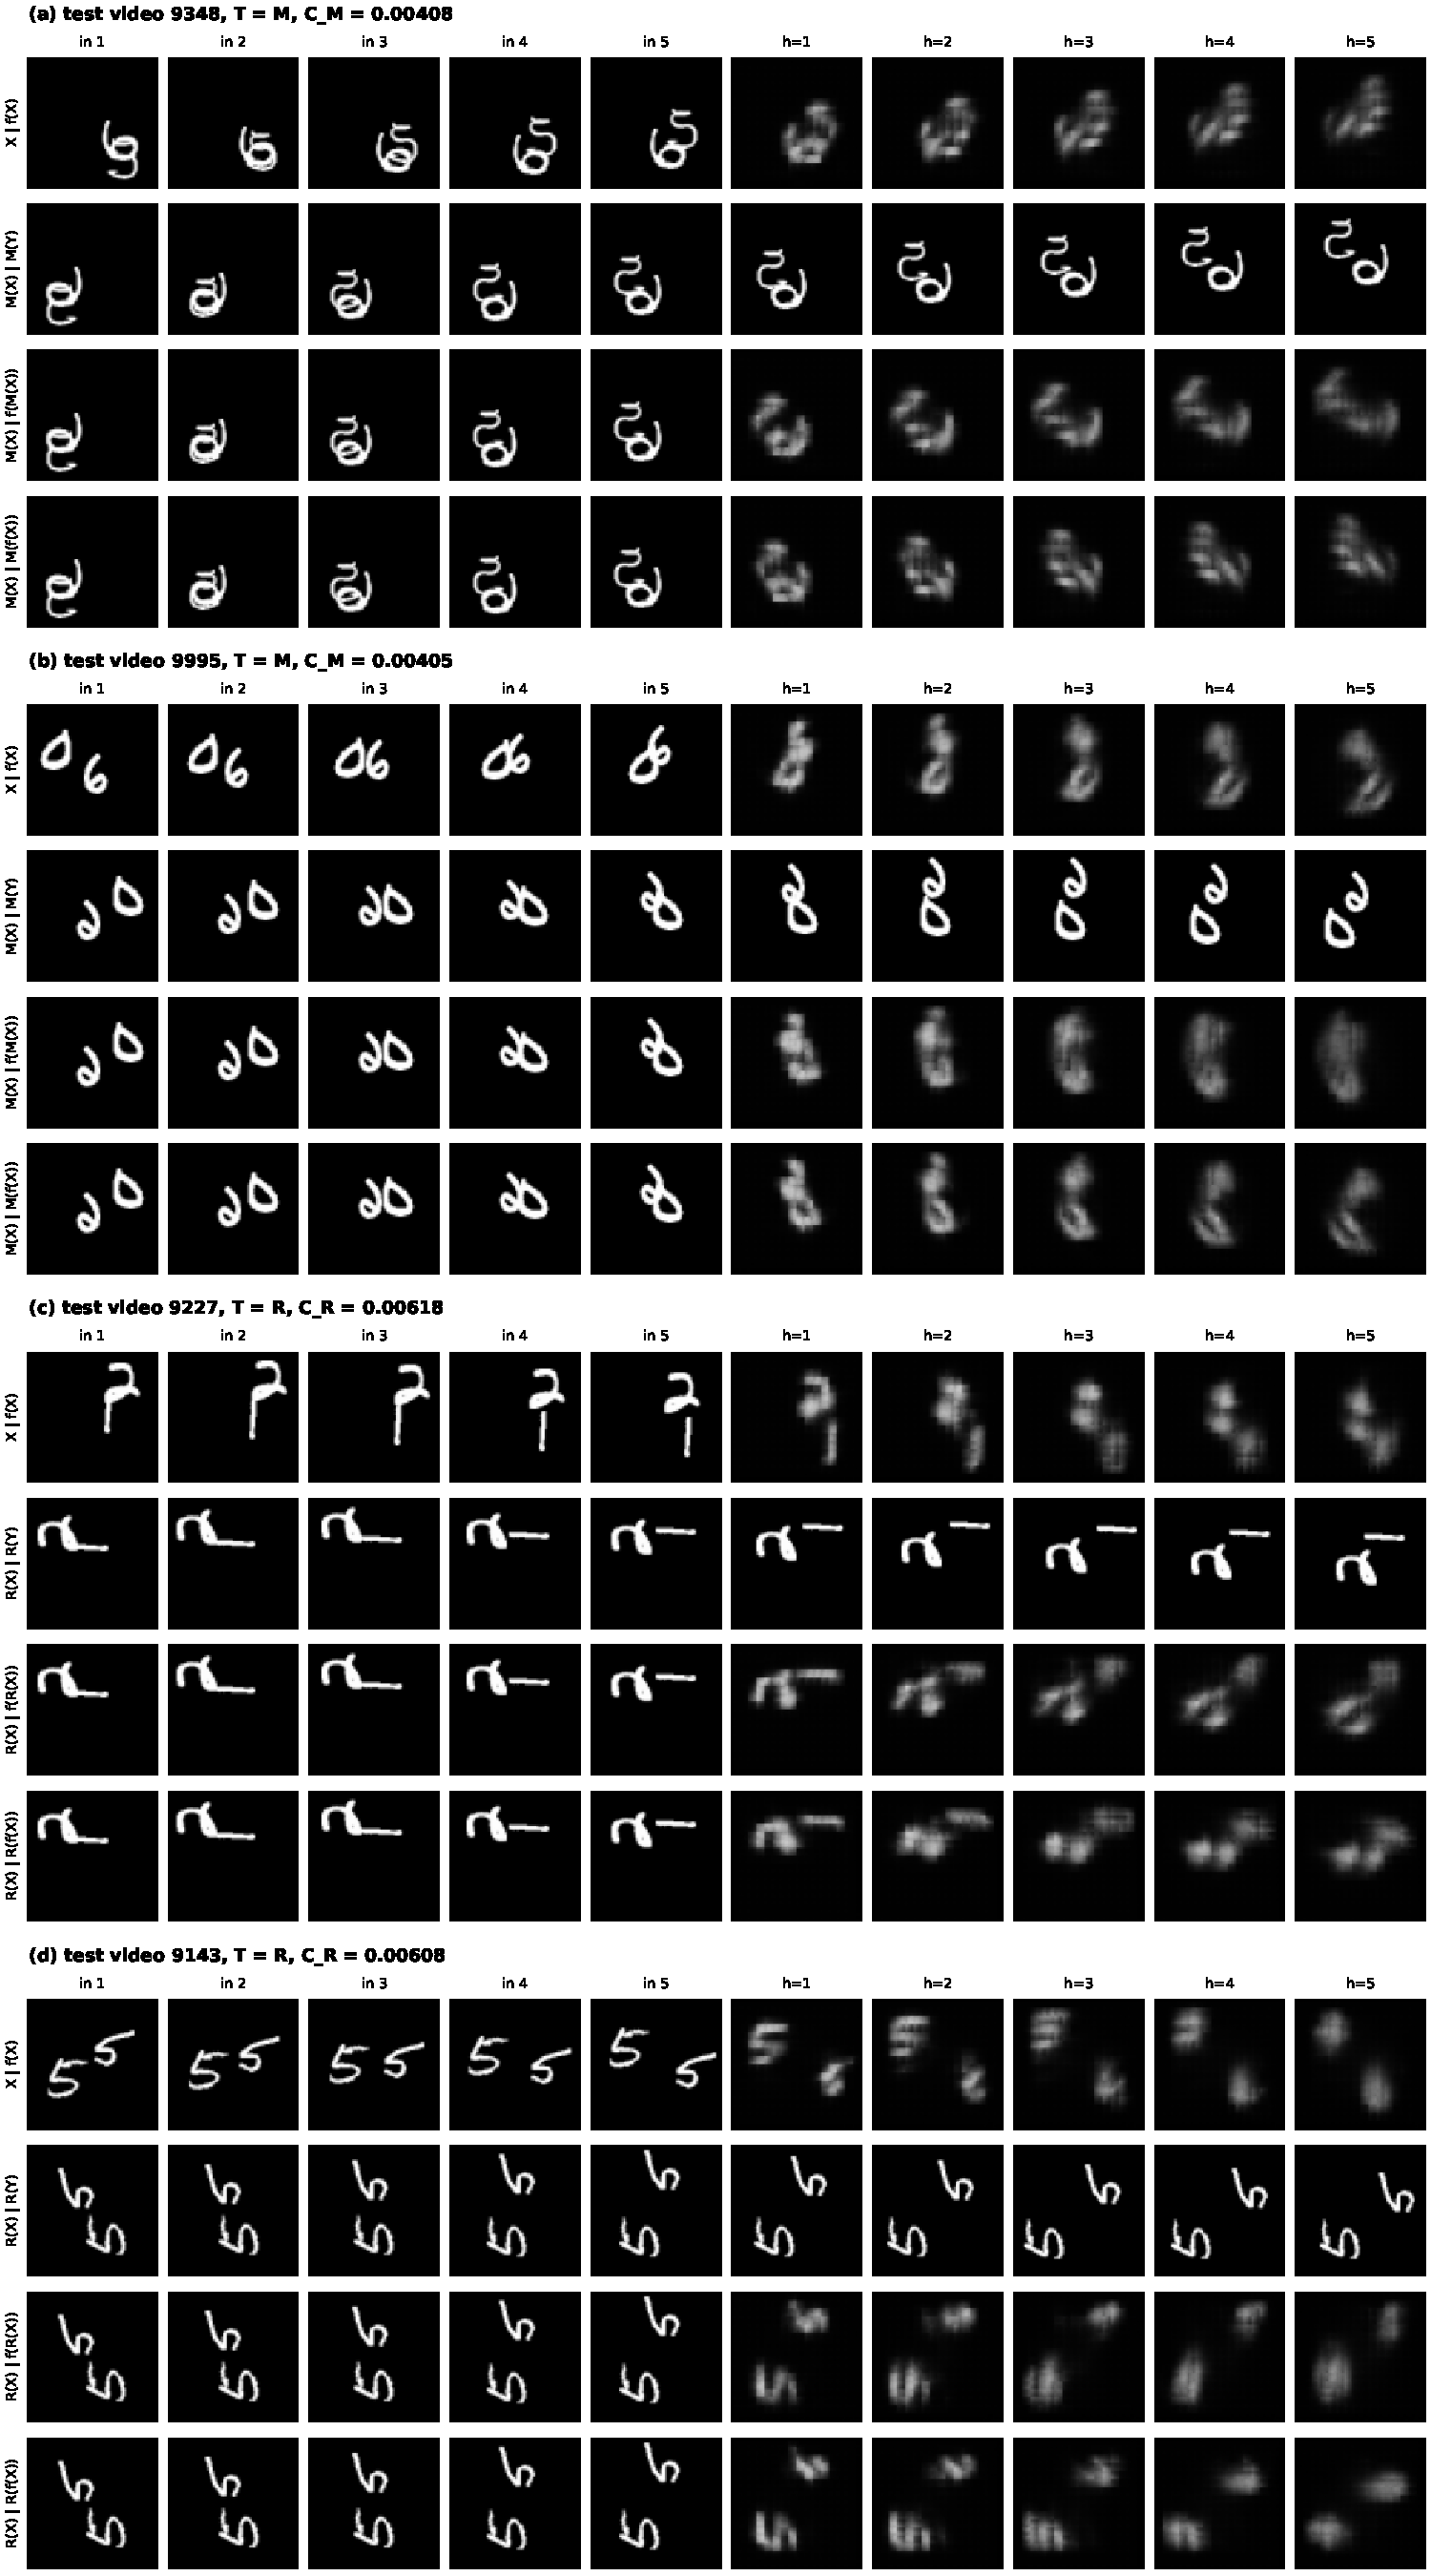
\includegraphics[height=0.86\textheight]{figures/figure3_symmetry_worst.pdf}
\caption{The two test videos with the largest per-video $C_M$ (a, b) and the
two with the largest $C_R$ (c, d), for seed-0 model A. Rows: (1) $X\,|\,f(X)$,
(2) $T(X)\,|\,T(Y)$, (3) $T(X)\,|\,f(T(X))$, (4) $T(X)\,|\,T(f(X))$. GIFs that
step through the five horizons:
\texttt{results/gifs/figure3a\_M\_video9348.gif},
\texttt{figure3b\_M\_video9995.gif}, \texttt{figure3c\_R\_video9227.gif},
\texttt{figure3d\_R\_video9143.gif}.}
\label{fig:q2-worst}
\end{figure}

\begin{figure}[H]
\centering
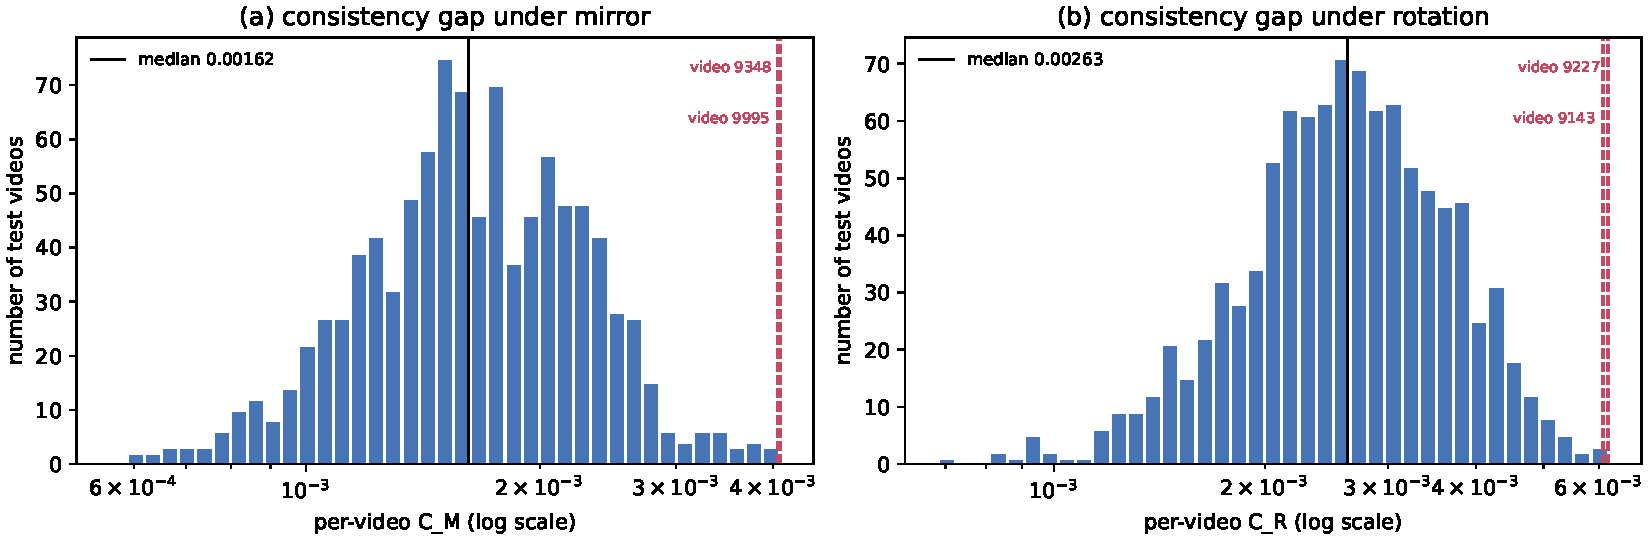
\includegraphics[width=\textwidth]{figures/figure4_consistency_hist.pdf}
\caption{Per-video $C_M$ (a) and $C_R$ (b) for seed-0 model A over the test
set (log scale), with the Figure~3 videos marked in red. The median $C_R$
(2.63e-03) is 1.6$\times$ the median $C_M$ (1.62e-03). The Figure~3 videos are
the extreme right tail, not typical cases.}
\label{fig:q2-hist}
\end{figure}

\paragraph{Q2.6.} Blank and Copy-last are exactly consistent because each one
commutes with \emph{any} pixel permutation. All-zero frames are zero in every
orientation, and copying the last frame commutes with flipping it. Yet they are
the two worst predictors in Table~3. So a small $C_T$ only says that a model
treats $T(X)$ the way it treats $X$. It says nothing about whether either
prediction is right. $C_T$ must always be read next to $E_T$:
\begin{itemize}
  \item a useful model needs \emph{small $C_T$ and small $E_T$};
  \item large $C_T$ means the rule depends on orientation;
  \item small $C_T$ with large $E_T$ means the model is consistently wrong.
\end{itemize}

\paragraph{Q2.7: video 9143, rotation; Figure 3(d) and its GIF.} The video
shows two 5s. After rotation, the upper digit moves up and to the right while
the lower one drifts slowly (row 2).
\begin{itemize}
  \item \textbf{Row 4} is the rotated version of the original forecast. It keeps
        \emph{both} digits as two blobs moving apart along the correct paths.
  \item \textbf{Row 3} is the forecast made from the rotated input. The upper
        digit thins out after $h=2$ and has largely \emph{vanished} by
        $h=4$--$5$: the model \emph{loses} it. The lower digit smears into a
        vertical streak rather than holding its shape.
\end{itemize}
The motion itself is not reversed or bounced. The model tracks a rotated 5
less confidently and lets its mass fade. On this video, rotation raises model
A's error from 0.0288 to 0.034, a \emph{correctness} loss as well as a
consistency gap ($C_R=$ 6.08e-03).

\paragraph{Q2.8.} Rotation is harder than mirroring, but only modestly:
\begin{itemize}
  \item $C_R=$ 2.98e-03 against $C_M=$ 1.83e-03 (1.6$\times$, in both seeds);
  \item $E_R=0.024$ against $E_M=0.023$, compared with $E^{(5)}=0.0224$.
\end{itemize}
The difference comes from \textbf{appearance, not motion}. Both transformations
map training directions to directions that occur in training, and neither
changes speed (Q2.1, Q2.2). But a mirror keeps digits upright, and several
digits (0, 1, 8) are nearly mirror-symmetric. A $90^\circ$ rotation turns every
digit on its side, which never happens in training. Model B confirms this
(Table~5): symmetry augmentation shows the model the transformed shapes without
changing the motion, and it halves $C_R$ (2.98e-03 to 1.58e-03) while bringing
$E_R$ down to $E^{(5)}$.

\begin{table}[H]
\centering\small
\caption{Speed test ($t=1$). $E^{(2)}$ is compared across speeds. For reference, Blank scores 0.0426 at every speed.}
\label{tab:q2-speed}
\resizebox{\textwidth}{!}{%
\begin{tabular}{@{}lccccc@{}}
\toprule
& $E^{(2)}$ $1\times$ & $E^{(2)}$ $2\times$ & $E^{(2)}$ $3\times$ & $E^{(5)}$ $1\times$ & $E^{(5)}$ $2\times$ \\
\midrule
Model A & 0.019 (0.0197, 0.0183) & \textbf{0.0456} (0.0453, 0.0459) & \textbf{0.0536} (0.0539, 0.0532) & 0.0224 (0.023, 0.0218) & 0.05 (0.0501, 0.0499) \\
Copy-last & 0.0548 & 0.0661 & 0.0703 & 0.0641 & 0.0719 \\
\bottomrule
\end{tabular}%
}
\end{table}

\begin{figure}[H]
\centering
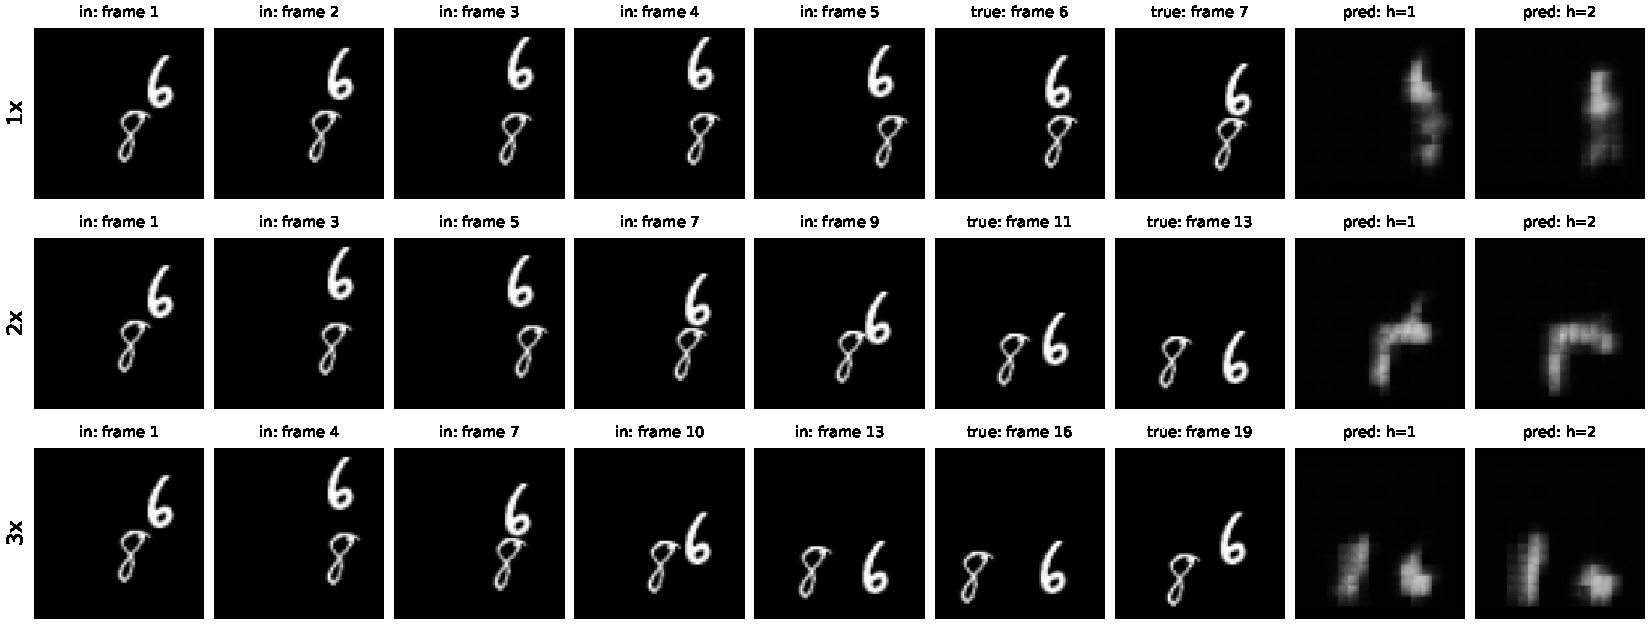
\includegraphics[width=\textwidth]{figures/figure5_speed.pdf}
\caption{Test video 9017 at $1\times$, $2\times$ and $3\times$ ($t=1$): the
five inputs, the first two true future frames, and seed-0 model A's first two
predictions. The digits are apart in every displayed true frame (checked by
connected components).}
\label{fig:q2-speed}
\end{figure}

\paragraph{Q2.9.} Model A falls apart \textbf{already at $2\times$}. Its
$E^{(2)}$ jumps 2.4$\times$, from 0.019 to 0.0456, which is \emph{worse than
predicting blank frames} (0.0426). At $3\times$ it gets worse again (0.0536).
This does \emph{not} agree with the reach estimate: 6.6\,px per frame is inside
the 8\,px reach, so $2\times$ should have been trackable. The estimate missed
two things:
\begin{enumerate}[label=(\roman*), leftmargin=*]
  \item \textbf{Reach is only an upper bound on what the architecture can
        express.} A learned model only uses the paths that training gave it a
        reason to use, and it never saw speeds above about 4.7\,px. So the
        relevant limit was the training distribution, not the architecture
        (tested in Q2.13).
  \item \textbf{The model must also infer velocity from the history.} At
        $2\times$, that history is unlike anything it has seen.
\end{enumerate}
What the failure looks like in Figure~5:
\begin{itemize}
  \item \textbf{At $2\times$,} the two digits are replaced by \emph{one blurred
        blob between them}. The model hedges, averaging over positions it
        cannot commit to, which is the MSE-optimal response to uncertainty.
  \item \textbf{At $3\times$,} it produces two blobs near the digits'
        \emph{last observed} positions: the digits \emph{stall}. The model
        falls back to blurred persistence, because it cannot connect the old
        position to the new one.
\end{itemize}
No digit is duplicated, and none vanishes completely.

\paragraph{Q2.10.} These results alone cannot tell the two causes apart. Fast
motion is both \emph{unfamiliar} (absent from training) and \emph{close to or
beyond reach} (6.6 and 10\,px against 8\,px), and both explanations predict
failure at $2\times$ and $3\times$. To separate them, change one factor at a
time:
\begin{enumerate}[leftmargin=*]
  \item \textbf{Same architecture, more data:} retrain the reach-8 architecture
        on speed-augmented windows (model C). If the error at a given speed
        drops, that failure was unfamiliarity. If $3\times$ stays bad, it is
        reach.
  \item \textbf{Same data, more reach:} train an architecture with larger reach
        on the same speed-augmented data (model D). If D fixes what C cannot,
        the remaining failure was architectural.
\end{enumerate}

% ---------------------------------------------------------------------------
\subsection{What Can Data Fix?}

\paragraph{Q2.11 (verbatim, committed at \texttt{cbe906a} before B, C, D were trained).}
\begin{quote}\small
Model B (symmetry augmentation) will shrink C\_M and C\_R and bring E\_M and E\_R down to about E(5), since the remaining mirror/rotation gap comes from digit appearance, but it will not help at $2\times$ or $3\times$. Model C (speed augmentation) will fix most of the $2\times$ failure, bringing E(2) at $2\times$ well below Blank, because 6.6 px per frame is within model A's 8 px reach and was only unfamiliar; at $3\times$ (about 10 px, beyond the reach) it will improve only partly. Model D (larger reach, also speed-augmented) will also fix $3\times$, with E(2) at $3\times$ clearly below model C's, while staying about as accurate as A at $1\times$.
\end{quote}

\begin{table}[H]
\centering\footnotesize
\caption{Models A--D on the test set. Training time: mean seconds per epoch over 30 epochs on the Tesla T4. Inference: seconds to predict all 1,000 test videos ($1\times$, $t=1$, batch 32) on the CPU.}
\label{tab:q2-datafix}
\resizebox{\textwidth}{!}{%
\begin{tabular}{@{}lccccc@{}}
\toprule
& $E^{(5)}$ $1\times$ & $C_M$ & $E_M$ & $C_R$ & $E_R$ \\
\midrule
A & 0.0224 (0.023, 0.0218) & 1.83e-03 (1.72e-03, 1.94e-03) & 0.023 (0.0235, 0.0225) & 2.98e-03 (2.74e-03, 3.22e-03) & 0.024 (0.0244, 0.0235) \\
B & 0.0221 (0.0228, 0.0215) & 1.37e-03 (1.47e-03, 1.28e-03) & 0.0222 (0.0228, 0.0215) & 1.58e-03 (1.62e-03, 1.53e-03) & 0.0221 (0.0228, 0.0215) \\
C & 0.0271 (0.0277, 0.0265) & 9.39e-04 (7.02e-04, 1.18e-03) & 0.0274 (0.0279, 0.0268) & 2.21e-03 (1.73e-03, 2.68e-03) & 0.0283 (0.0287, 0.0279) \\
D & 0.0269 (0.0265, 0.0274) & 7.15e-04 (8.72e-04, 5.58e-04) & 0.0271 (0.0267, 0.0275) & 1.95e-03 (2.09e-03, 1.82e-03) & 0.0281 (0.0278, 0.0284) \\
\bottomrule
\end{tabular}%
}

\vspace{6pt}
\resizebox{\textwidth}{!}{%
\begin{tabular}{@{}lcccccc@{}}
\toprule
& $E^{(2)}$ $1\times$ & $E^{(2)}$ $2\times$ & $E^{(2)}$ $3\times$ & Params & Train (s/epoch) & Inference (s) \\
\midrule
A & 0.019 (0.0197, 0.0183) & 0.0456 (0.0453, 0.0459) & 0.0536 (0.0539, 0.0532) & 480,784 & 10.3 (10.3, 10.3) & 9.64 (8.76, 10.5) \\
B & 0.0185 (0.0189, 0.018) & 0.0446 (0.0444, 0.0447) & 0.0497 (0.0506, 0.0489) & 480,784 & 11.3 (11.1, 11.4) & 10.7 (10.6, 10.9) \\
C & 0.0233 (0.0239, 0.0228) & 0.0289 (0.0293, 0.0284) & 0.0336 (0.0335, 0.0336) & 480,784 & 10.7 (10.7, 10.7) & 9.61 (9.64, 9.57) \\
D & 0.0242 (0.0237, 0.0247) & 0.029 (0.0288, 0.0291) & 0.0326 (0.0325, 0.0327) & 480,784 & 16.1 (16.1, 16.1) & 10.3 (9.56, 11.1) \\
\bottomrule
\end{tabular}%
}
\end{table}

\paragraph{Q2.12: model D.}
\begin{itemize}
  \item \textbf{The design.} Model D is model A with the layer-2 ConvLSTM
        convolution \textbf{dilated by 2} (kernel $3\times3$, padding 2). Every
        other part is identical: shapes, rollout, training protocol, and
        parameter count (\textbf{480,784}, against a limit of 721,176).
  \item \textbf{Its reach} is calculated exactly as in Q2.3. The longest path
        within a step still enters at layer 1 (from $u_\tau$ or
        $h^{(1)}_{\tau-1}$). It moves 1 cell in the layer-1 convolution and
        $2\times\lfloor 3/2\rfloor=2$ cells in the dilated layer-2 convolution.
        So $\text{reach}=4\times(1+2)=\textbf{12 px}>8$\,px, which is strictly
        larger.
  \item \textbf{Why this candidate.} Layer 1 is undilated, so the offsets
        reachable in one step still cover every cell up to 3 away. A model
        dilated in both layers covers only even offsets.
\end{itemize}
\emph{How it was chosen: on the validation split only} (videos 8,000--8,999).
Four candidates were trained like model C (seed 0), and we picked the lowest
mean validation $E^{(2)}$ over $1\times$, $2\times$ and $3\times$:

\begin{center}\footnotesize
\resizebox{\textwidth}{!}{%
\begin{tabular}{@{}lllccccc@{}}
\toprule
Candidate & Change from A & Params & Reach & val $E^{(2)}$ $1\times$ & $2\times$ & $3\times$ & mean \\
\midrule
(C, reference) & -- & 480,784 & 8 px & 0.0237 & 0.0292 & 0.033 & 0.0286 \\
\textbf{Ddil12} & layer-2 dilation 2 & 480,784 & 12 px & \textbf{0.0236} & \textbf{0.029} & 0.032 & \textbf{0.0282} \\
Ddil22 & both dilations 2 & 480,784 & 16 px & 0.0264 & 0.0297 & \textbf{0.0318} & 0.0293 \\
Dpatch8 & $8\times8$ patches & 594,496 & 16 px & 0.0395 & 0.0395 & 0.0395 & 0.0395 \\
D3layer & 3 layers, 56 channels & 598,320 & 12 px & 0.0395 & 0.0395 & 0.0395 & 0.0395 \\
\bottomrule
\end{tabular}%
}
\end{center}
\noindent Dpatch8 and D3layer \emph{collapsed} during the first epoch: they
output the same faint mean frame for every video, and they never recovered
under the fixed protocol (Adam $10^{-3}$, 30 epochs). That itself rules them
out, because model D must train reliably under that protocol.

\paragraph{Q2.13: labelling the failures.}
\begin{itemize}
  \item \textbf{Mirror and rotation gaps: appearance.} B changes only what the
        model sees (transformed digits, the same $1\times$ motion). It cuts
        $C_R$ from 2.98e-03 to 1.58e-03 and $C_M$ from 1.83e-03 to 1.37e-03,
        and brings $E_M$ and $E_R$ (0.0222 and 0.0221) to $E^{(5)}$ (0.0221),
        while its speed errors stay close to A's ($2\times$: 0.0446). C and D
        also lower $C_M$, but with a higher $E_M$, so they are more consistent
        without being more correct.
  \item \textbf{The $2\times$ failure: unfamiliar motion.} C keeps A's
        architecture and reach and only adds fast training windows. That alone
        cuts $E^{(2)}$ at $2\times$ from 0.0456 to \textbf{0.0289}, far below
        Blank (0.0426). D adds nothing at $2\times$ (0.029).
  \item \textbf{The $3\times$ failure: mostly unfamiliar motion, with a small
        architectural-reach part.} C cuts $3\times$ from 0.0536 to 0.0336. D's
        extra reach lowers it further only to \textbf{0.0326}. That 3\% gain is
        consistent across seeds (0.0335 and 0.0336 for C, against 0.0325 and
        0.0327 for D), but small.
\end{itemize}
So the hypothetical in the handout ("C still bad at $3\times$, D good") did
\emph{not} occur here. Had it occurred, it would have shown a pure reach
limit: within one update, the output at a digit's new position is a function
\emph{only} of inputs and states within the reach. If the digit's old position
lies outside that neighbourhood, no setting of the weights can connect the
two. More data changes the weights, not the computation graph, so it cannot
create a path the architecture does not contain; the model can only hedge, by
blurring or stalling.

C copes at $3\times$ despite 10\,px exceeding the 8\,px reach for two reasons.
First, digits are about 20\,px wide, so parts of the old and new digit lie
within reach of each other. Second, the reach is measured centre to centre in
the 4-pixel-wide folded cells, so it is not a hard wall at exactly 8\,px. This
is why reach mattered far less than familiarity. Our Q2.11 prediction was
right about B and C, but too optimistic about how much D would add at
$3\times$.

\paragraph{Q2.14.} \textbf{Yes, speed augmentation cost $1\times$ accuracy.}
\begin{itemize}
  \item $E^{(5)}$ at $1\times$ rises from 0.0224 (A) to 0.0271 (C) and 0.0269
        (D), about +20\%. $E^{(2)}$ at $1\times$ rises from 0.019 to 0.0233 and
        0.0242.
  \item The same capacity must now cover three speeds, and only a third of the
        training windows are at $1\times$.
  \item Symmetry augmentation cost nothing: B is slightly \emph{better} than A
        at $1\times$ (0.0221).
\end{itemize}
Whether the trade is worth it depends on use:
\begin{itemize}
  \item If test-time speed varies, it is clearly worth it. C and D cut the error
        at $2\times$ and $3\times$ by 36--39\%, turning a worse-than-Blank
        model into one well below Blank. They lose 20\% only at the speed where
        A was already good.
  \item If every clip is guaranteed to be $1\times$, A or B is preferable.
\end{itemize}

% ---------------------------------------------------------------------------
\subsection{The Final Model}

\paragraph{Symmetrisation is exactly consistent.} Each $g\in G$ is a pixel
permutation, so it is linear, and $g$ commutes with averaging. Let
$h\in G$. Then
\[
  \bar f(hX)=\tfrac18\sum_{g\in G} g^{-1} f(ghX)
  =\tfrac18\sum_{g'\in G} h\,g'^{-1} f(g'X)
  =h\,\bar f(X),
\]
where we substituted $g'=gh$, so that $g^{-1}=h\,g'^{-1}$. As $g$ runs over the
group $G$, so does $g'$, because right-multiplication by $h$ is a bijection of
$G$. Hence $\bar f(T(X))=T(\bar f(X))$ for every $T\in G$, and
$C_M=C_R=0$ exactly, for \emph{any} $f$.

It follows that $E_T=\mathrm{MSE}(T\bar f(X),T(Y))=\mathrm{MSE}(\bar f(X),Y)$,
because a permutation does not change a pixel-averaged error. So $E_M=E_R=E^{(5)}$.
Numerically, we measure 4.8e-17 to 9.3e-17 (Table~6), which is floating-point
rounding.

\paragraph{Choice of final model: symmetrised D} (not D+B).
\begin{itemize}
  \item In Table~5, symmetry augmentation helped only consistency, plus a
        marginal gain at $1\times$ (B against A: 0.0221 against 0.0224).
        Symmetrisation makes consistency exact anyway.
  \item Training D+B would cost two more runs without targeting a remaining
        failure.
  \item D is the most speed-robust model, and the wrapper adds the symmetry.
\end{itemize}

\begin{table}[H]
\centering\footnotesize
\caption{Symmetrised models (test set). The training time is that of the underlying learned model; symmetrisation needs no training. Inference includes all 8 transforms, forward passes, inverse transforms and the averaging.}
\label{tab:q2-final}
\resizebox{\textwidth}{!}{%
\begin{tabular}{@{}lccccc@{}}
\toprule
& $E^{(5)}$ $1\times$ & $C_M$ & $E_M$ & $C_R$ & $E_R$ \\
\midrule
Symm.\ B & 0.0215 (0.0221, 0.0209) & 9.27e-17 (8.99e-17, 9.56e-17) & 0.0215 (0.0221, 0.0209) & 7.49e-17 (7.28e-17, 7.70e-17) & 0.0215 (0.0221, 0.0209) \\
\textbf{Symm.\ D (final)} & 0.0269 (0.0265, 0.0274) & 6.14e-17 (6.62e-17, 5.65e-17) & 0.0269 (0.0265, 0.0274) & 4.83e-17 (5.34e-17, 4.32e-17) & 0.0269 (0.0265, 0.0274) \\
\bottomrule
\end{tabular}%
}

\vspace{6pt}
\resizebox{\textwidth}{!}{%
\begin{tabular}{@{}lcccccc@{}}
\toprule
& $E^{(2)}$ $1\times$ & $E^{(2)}$ $2\times$ & $E^{(2)}$ $3\times$ & Params & Train (s/epoch) & Inference (s) \\
\midrule
Symm.\ B & 0.018 (0.0185, 0.0176) & 0.0438 (0.0438, 0.0437) & 0.0486 (0.0496, 0.0476) & 480,784 & 11.3 (11.1, 11.4) & 75 (75.5, 74.5) \\
\textbf{Symm.\ D (final)} & 0.0242 (0.0237, 0.0248) & 0.029 (0.0288, 0.0292) & 0.0326 (0.0325, 0.0327) & 480,784 & 16.1 (16.1, 16.1) & 85.9 (90.9, 80.8) \\
\bottomrule
\end{tabular}%
}
\end{table}

\begin{figure}[p]
\centering
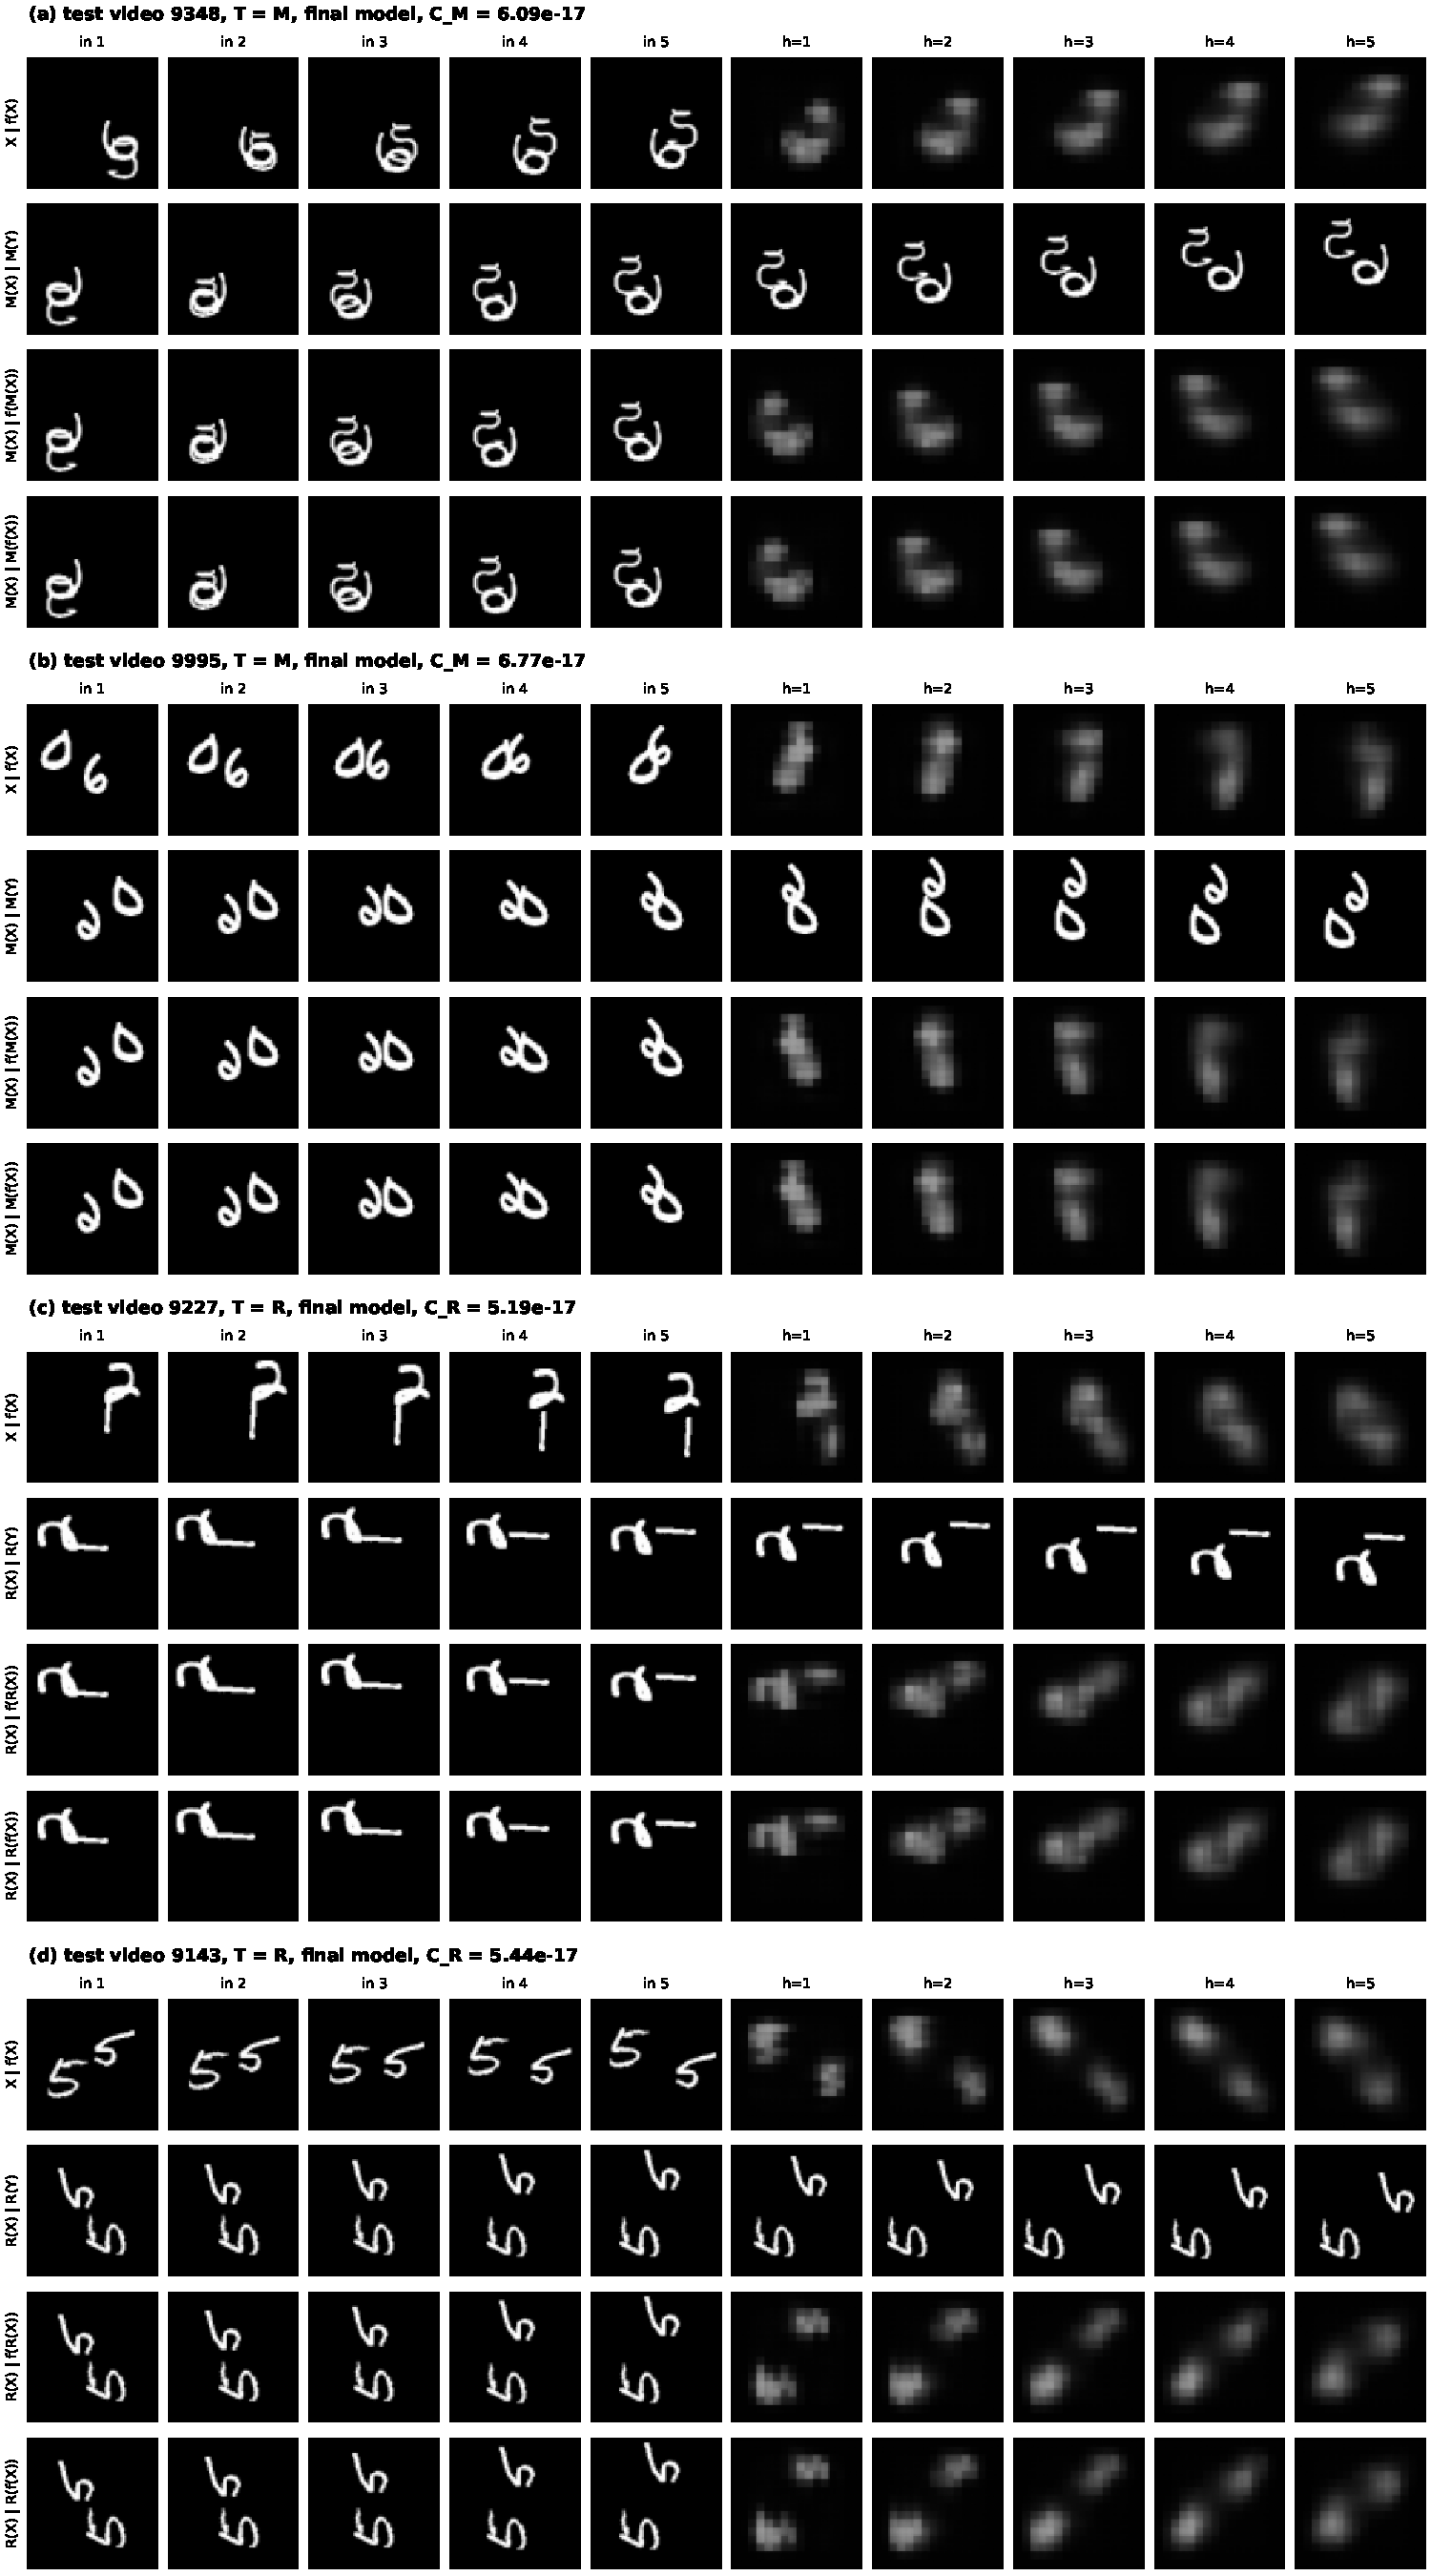
\includegraphics[height=0.62\textheight]{figures/figure6a_final_symmetry.pdf}\\[4pt]
\textbf{(a)}\\[6pt]
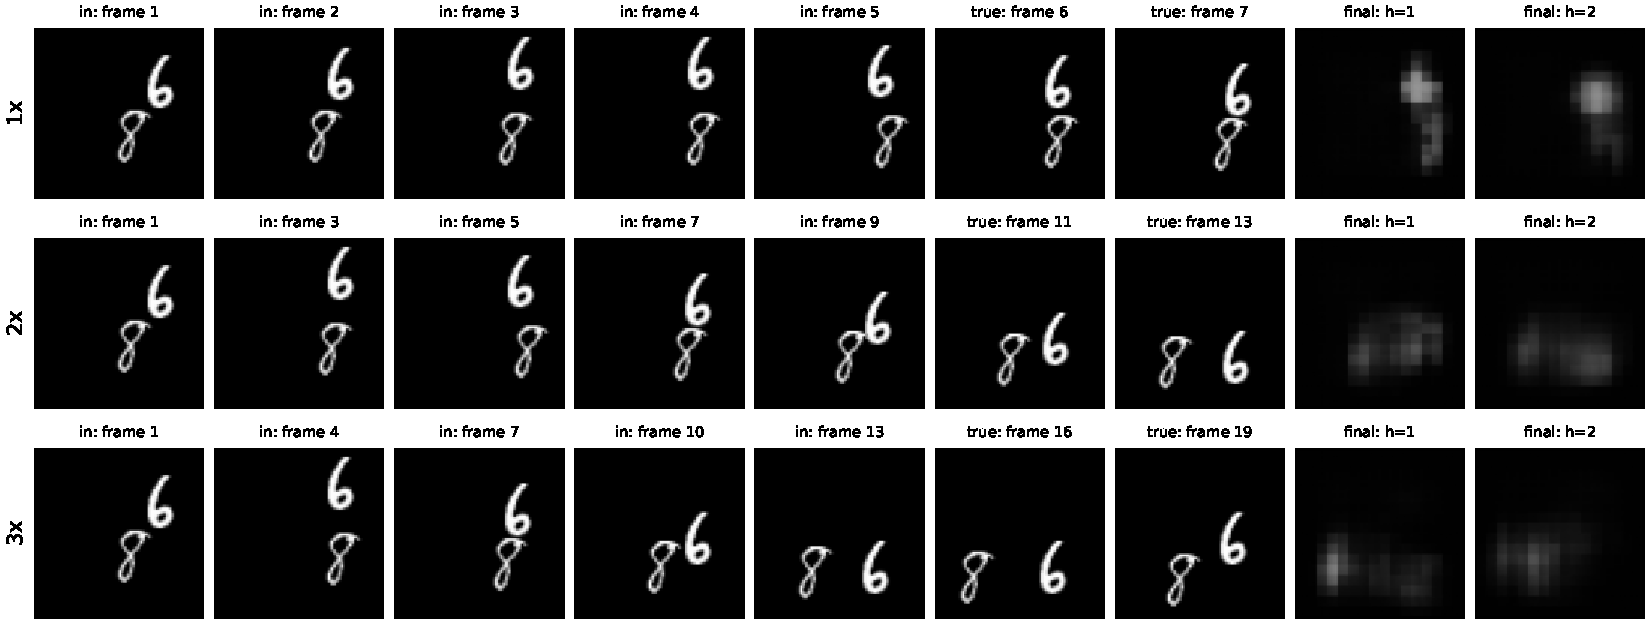
\includegraphics[width=\textwidth]{figures/figure6b_final_speed.pdf}\\[2pt]
\textbf{(b)}
\caption{The final model (symmetrised seed-0 D). (a) Figure~3 repeated on the
same four videos: rows 3 and 4 now coincide, with per-video $C$ between 5e-17
and 7e-17. GIFs: \texttt{results/gifs/figure6a-a\_M\_video9348\_final.gif},
\texttt{figure6a-b\_M\_video9995\_final.gif},
\texttt{figure6a-c\_R\_video9227\_final.gif},
\texttt{figure6a-d\_R\_video9143\_final.gif}. (b) Figure~5 repeated on test
video 9017.}
\label{fig:q2-finalfig}
\end{figure}

\paragraph{Q2.15: learned versus built-in symmetry.}
\begin{itemize}
  \item \textbf{Consistency.} Learned symmetry (B) only \emph{reduces} the gaps,
        to $C_M=$ 1.37e-03 and $C_R=$ 1.58e-03. Built-in symmetry is
        \textbf{exact} (below 1e-16), because it holds by construction for any
        weights (proof above). Augmentation only rewards consistency on the
        training distribution, through a finite number of gradient steps.
  \item \textbf{Accuracy.} Symmetrising \emph{improved} B at $1\times$ (0.0221
        to 0.0215) and at $2\times$ and $3\times$ (0.0446 to 0.0438, and
        0.0497 to 0.0486). It left D unchanged (0.0269, 0.029, 0.0326). On
        transformed clips, the symmetrised models' $E_M=E_R=E^{(5)}$ exactly,
        whereas B's are 0.0222 and 0.0221.
  \item \textbf{Inference cost.} Symmetrising costs 8 forward passes: 75\,s
        against 10.7\,s for B, and 85.9\,s against 10.3\,s for D (about
        7--8$\times$). Learned symmetry is free at test time.
  \item \textbf{When averaging hurts.} Averaging hurts when the 8 predictions
        are individually sharp but \emph{disagree}, for example a model that is
        confident about upright digits but wrong about rotated ones. The
        average then ghosts, or blurs a sharp correct prediction with wrong
        ones.
\end{itemize}
Here it did not hurt MSE. An MSE-trained model's predictions are already
blurred conditional means, so averaging mainly reduces variance, like an
ensemble. The gain appears for B, which was trained on all 8 orientations, so
each of its views is about equally good. D never saw rotated digits: its
rotated views are worse, and that cancels the ensemble gain. It did
cost \emph{sharpness}: in Figure~6(b) the final model's digits are softer than
model A's in Figure~5, and at $1\times$ the 8 fades, which MSE does not
penalise heavily.

\paragraph{Q2.16: back to video 9143 (Figure 6(a)(d)).}
\begin{itemize}
  \item \textbf{The inconsistency is fixed.} Rows 3 and 4 are now identical
        ($C_R=$ 5.44e-17, against 6.08e-03 for A). The upper digit no longer
        vanishes: both digits persist as two blobs moving apart, as in the
        ground truth.
  \item \textbf{Which change fixed it:} \textbf{symmetrisation} fixed the
        consistency and the vanishing digit. The rotated input is averaged with
        the views in which the digits look familiar.
  \item \textbf{Speed augmentation and reach} (the changes from A to D) play no
        part on a $1\times$ clip. They slightly reduce sharpness at $1\times$:
        D's own error on this video is 0.0314, against 0.0288 for A.
  \item \textbf{Is it fully right?} Not quite. The rotated error falls from
        0.034 (A) to 0.0321, but the digits are still blurry blobs and lose
        their identity after about $h=2$. So the \emph{motion} is now right,
        and the \emph{appearance} is not.
\end{itemize}

\paragraph{Q2.17: final verdict.} Partly. The final model has learned a
transferable motion rule, not just training-set memory:
\begin{itemize}
  \item it is exactly consistent under all 8 symmetries, with $E_T=E^{(5)}$;
  \item after speed augmentation it tracks digits at $2\times$ and $3\times$,
        cutting A's error there by about 37\%;
  \item it extrapolates direction and bounces correctly for the first horizons.
\end{itemize}
But consistency was \emph{imposed} by construction, and speed robustness came
from \emph{seeing} fast motion in training, not from inferring it. A skeptic
would want generalisation to conditions \emph{never} trained on: unseen speeds
(say $1.5\times$ or $4\times$), longer rollouts, or new shapes moving under the
same rule. One test it has clearly not passed is \textbf{keeping the digits
sharp and identifiable for five steps}. Predictions blur into blobs by
$h=3$--$5$, and overlapping digits merge. So the model carries positions and
velocities, but not appearance.


\clearpage
{\small
\begin{thebibliography}{99}\setlength{\itemsep}{0pt}
\bibitem{tcn} S.~Bai, J.~Z. Kolter, V.~Koltun. An empirical evaluation of generic convolutional and recurrent networks for sequence modeling. \emph{arXiv:1803.01271}, 2018.
\bibitem{transformer} A.~Vaswani et al. Attention is all you need. \emph{NeurIPS}, 2017.
\bibitem{koenker} R.~Koenker, G.~Bassett. Regression quantiles. \emph{Econometrica} 46(1), 1978.
\bibitem{tft} B.~Lim, S.~\"O. Ar{\i}k, N.~Loeff, T.~Pfister. Temporal Fusion Transformers for interpretable multi-horizon time series forecasting. \emph{Int.\ J.\ Forecasting} 37(4), 2021.
\bibitem{dcrnn} Y.~Li, R.~Yu, C.~Shahabi, Y.~Liu. Diffusion convolutional recurrent neural network: data-driven traffic forecasting. \emph{ICLR}, 2018.
\bibitem{gwn} Z.~Wu, S.~Pan, G.~Long, J.~Jiang, C.~Zhang. Graph WaveNet for deep spatial-temporal graph modeling. \emph{IJCAI}, 2019.
\bibitem{kratzert} F.~Kratzert et al. Rainfall--runoff modelling using Long Short-Term Memory (LSTM) networks. \emph{Hydrology and Earth System Sciences} 22, 2018.
\bibitem{chow} V.~T. Chow, D.~R. Maidment, L.~W. Mays. \emph{Applied Hydrology}. McGraw-Hill, 1988.
\bibitem{cqr} Y.~Romano, E.~Patterson, E.~Cand\`es. Conformalized quantile regression. \emph{NeurIPS}, 2019.
\bibitem{shi} X.~Shi, Z.~Chen, H.~Wang, D.-Y. Yeung, W.-K. Wong, W.-C. Woo. Convolutional LSTM network: a machine learning approach for precipitation nowcasting. \emph{NeurIPS}, 2015.
\bibitem{srivastava} N.~Srivastava, E.~Mansimov, R.~Salakhutdinov. Unsupervised learning of video representations using LSTMs. \emph{ICML}, 2015.
\end{thebibliography}
}

% ===========================================================================
\section*{Generative AI usage disclosure}
% ===========================================================================
{\small
\textbf{Tool:} Claude (Anthropic), used through Claude Code in VS Code, for
both questions.

\textbf{What it produced:}
\begin{itemize}
  \item an explanation of the assignment;
  \item the Q1 solution approach and the full Q1 write-up (LaTeX and TikZ
        figures);
  \item guidance on the companion notebook;
  \item all Q2 code (\texttt{q2/}, \texttt{colab/train\_q2.ipynb}), which it
        tested on the local machine;
  \item the GitHub setup and commits;
  \item model D's candidates and its validation-only selection;
  \item all Q2 tables, figures and GIFs, produced by running the code;
  \item drafts of the Q2.5 and Q2.11 predictions, written before the
        corresponding experiments, then reviewed and approved by the student
        and committed unedited;
  \item drafts of all other Q2 answers;
  \item this combined report.
\end{itemize}
Training ran on Google Colab, launched by the student.

\textbf{Edits made by the student:}
\textcolor{red}{\textbf{[describe what you changed, checked or rewrote -- e.g.\ reviewed Q2.5/Q2.11 before committing, verified figures, reworded answers]}}

\textbf{Prompts (verbatim, in order):}
\begin{enumerate}[leftmargin=*,itemsep=0pt]
  \item ``this is the assignment document, that explains what the problem statement is, what is required to do and what is already provided. Please read this doc thoroughly and explain to me..''
  \item ``lets start with question 1. please explain how will we solve it ?''
  \item ``so you're saying, I need to run Question1/Question1.ipynb . Do I need to odify anything in that or is it good to run?''
  \item ``to run that notebook on google colab, what do i need to do ?''
  \item ``let me run it on my mac then''
  \item ``why did it open a localhost ?''
  \item ``so I run the notebook. Was ZI supposed to change anything ?''
  \item ``tell me step by step what i need to do''
  \item ``how do test the four prompts?''
  \item ``for each prompt, what do I need to do in the notebook ?''
  \item ``You have to write me complete report for question 1. Tell me what you need from me?''
  \item ``name: Muhammad Sikander Raheem, roll Number: 25280017, no github repolink yet. please use latex/overleaf. For architecture use defaults. Please write the report and I'll compile it in overleaf''
  \item ``This is a 12 page report. Can you please make it 7-9 pages''
  \item ``lets start question no 2 now. Tell me step by step how to do it and what you require from my side ?''
  \item ``what doi i need to push to repo ?''
  \item ``Which repo should I upload on github ?''
  \item ``so I'm using a github with a different email address. Do I just give you thye repo link ?''
  \item ``https://github.com/sikanderraheem21/DL4TSG\_PA2.git Here's the repo link''
  \item ``push''
  \item ``why is only this in the repo ?'' (with a screenshot of the repository)
  \item ``which will be fatser to train on, mac or colab?''
  \item ``Lets do with colab''
  \item ``we dont have to push anything to github hyet ?''
  \item ``what was it that sir required to be pushed to github before I started tarining ?''
  \item ``so now I open @colab/train\_q2.ipynb in colab and start running cells? Do I need to upload something on google drive ?''
  \item ``first I will run this notebook and then share results with you and then you will create another notebopok ?''
  \item ``Phase 2: model A only. Models B, C and D are trained in Phase 4, after the Q2.11 prediction has been committed. There is this comment in the notebook. what does it mean ?''
  \item ``and how do I change the runs ?''
  \item (screenshot of Colab training output) ``Training runs in progress''
  \item ``I have downloaded q2 results zip folder. should I add it in this workspaCE $>$?''
  \item ``what do i do now ?''
  \item ``what is the next step ?''
  \item ``can you write answer to 2.5 and review it from me''
  \item ``commit''
  \item ``do i have to train runs B C D on colab now ?''
  \item ``okay go ahaead''
  \item ``please draft answer for 2.11''
  \item ``commit''
  \item ``why are we oushing it ?'' (when a push was proposed), then ``push''
  \item ``So KI have run the updated colab notebook and the results are also downloaded. Can you tell me why you're making figures behind the scenes and not in the notebook itself ?''
  \item ``I have changed the github user''
  \item ``Run cells 1--4. Cell 3 pulls the update that makes Ddil12 model D. In the colab notebook, cell 3 is getting data from github''
  \item ``I have executed the notebook and the results folder is also downloaded''
  \item ``has the evaluation completed ?''
  \item ``please create a single report for Q1 and 2''
\end{enumerate}
}

\end{document}
